\documentclass[xcolor=svgnames, compress]{beamer}
%\documentclass[compress,red]{beamer}

\mode<presentation>

\usepackage{amsmath}

\usepackage{ragged2e}


\usepackage{comment}
\usepackage{multirow}
\usepackage{amsmath, amssymb}
\usepackage{graphicx}
\usepackage{color}

\usepackage{xcolor}


%\usepackage{arydshln}
\usepackage{marvosym}

\usepackage{hyperref}


\usepackage{booktabs, tabu}

\usepackage{tikz}
\usetikzlibrary{arrows,shapes,trees}
\usetikzlibrary{matrix}
\usetikzlibrary{calc}
\usepackage{tabularx}

\usepackage[T1]{fontenc}
\usepackage{mathpazo}

\usepackage{hhline}% http://ctan.org/pkg/hhline


%\includepackage{multimedia}

%\documentclass[draft]{beamer}
%\documentclass[compress]{beamer}
%\documentclass[xcolor=pst]{beamer}
%\usenavigationsymbolstemplate{}
%\setbeamertemplate{navigation symbols}{} 







\usetheme{UniversiteitAntwerpen}
%\usetheme{Ilmenau}
%\usetheme{Frankfurt}
%\usetheme{Amsterdam}
%\usetheme{Warsaw}


%\usetheme{Darmstadt}
%\useoutertheme{miniframes}
%\makeatletter
%  \beamer@compresstrue
%\makeatother



\setbeamercovered{transparent}


\useinnertheme{rounded}
\setbeamertemplate{items}[ball]
\setbeamertemplate{blocks}[rounded][shadow=true]
\setbeamertemplate{navigation symbols}{}
\setbeamercolor{normal text}{fg=Black}



\newtheorem{idef}{Intuitive Definition}



\newtheorem{goal}{Goal}
\newtheorem{nt}{Note}

\newtheorem{axioms}{Axioms}
\newtheorem{rl}{Rule}

\newtheorem{prop}{}

\newtheorem{pmf}{Probability Mass Function}



\newenvironment{changemargin}[2]{%
\begin{list}{}{%
\setlength{\topsep}{0pt}%
\setlength{\leftmargin}{#1}%
\setlength{\rightmargin}{#2}%
\setlength{\listparindent}{\parindent}%
\setlength{\itemindent}{\parindent}%
\setlength{\parsep}{\parskip}%
}%
\item[]}{\end{list}}


\newcommand*\circled[1]{\tikz[baseline=(char.base)]{
            \node[shape=circle,draw,inner sep=2pt] (char) {#1};}}

\newcommand*\dash{\rotatebox{90}{\Kutline} }


\usepackage{array}
\newcolumntype{L}[1]{>{\raggedright\let\newline\\\arraybackslash\hspace{0pt}}m{#1}}
\newcolumntype{C}[1]{>{\centering\let\newline\\\arraybackslash\hspace{0pt}}m{#1}}
\newcolumntype{R}[1]{>{\raggedleft\let\newline\\\arraybackslash\hspace{0pt}}m{#1}}



\newcommand*\dashline{\rotatebox[origin=c]{90}{$\dabar@\dabar@\dabar@$}}



\DeclareRobustCommand{\rchi}{{\mathpalette\irchi\relax}}
\newcommand{\irchi}[2]{\raisebox{\depth}{$#2\chi$}}




%\setbeamertemplate{headline}{%
%\leavevmode%
%  \hbox{%
%    \begin{beamercolorbox}[wd=\paperwidth,ht=3.5ex,dp=12.125ex]{palette quaternary}%
%    \insertsectionnavigationhorizontal{\paperwidth}{}{\hskip0pt plus1filll}
%    \end{beamercolorbox}%
%  }
%}




\AtBeginSection[]
{
\begin{frame}<beamer>{Table of Contents}
   %\begin{frame}
        %\frametitle{Inhalts\"ubersicht}
        %\frametitle{Inhalts\"ubersicht}
	\small        
        \tableofcontents[currentsection,currentsubsection]
	\normalsize
   \end{frame}
}







\makeatletter
  \beamer@compressfalse
\makeatother


\title{2. Descriptive Statistics\\
\vspace*{-0.25cm}
{\normalsize{STAT*2060: Statistics for Business Decisions} } }
\author{Nishan Mudalige}
\institute{Department of Mathematics and Statistics\\
University of Guelph}
\date[STAT*2080F14]{Fall 2014}

\begin{document}

\small

%\frame{\titlepage}

\begin{frame}
\vspace{0.25cm}
\maketitle



%\vspace*{0.60cm}
\hspace*{-0.25cm}
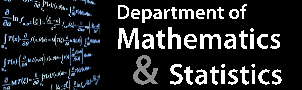
\includegraphics[width=2.75cm]{logo_UA_tekst_kl.pdf}

\end{frame}


\begin{frame}
\frametitle{Table of Contents}
\tableofcontents
\end{frame}


%\documentclass[xcolor=svgnames, compress, red]{beamer}
%%\documentclass[compress,red]{beamer}
%
%\mode<presentation>
%
%\usepackage{amsmath}
%
%\usepackage{ragged2e}
%
%
%\usepackage{comment}
%\usepackage{multirow}
%\usepackage{amsmath, amssymb}
%\usepackage{graphicx}
%\usepackage{color}
%
%\usepackage{xcolor}
%
%%\usepackage{arydshln}
%\usepackage{marvosym}
%
%\usepackage{hyperref}
%
%
%\usepackage{booktabs, tabu}
%
%\usepackage{tikz}
%\usetikzlibrary{arrows,shapes,trees}
%\usetikzlibrary{matrix}
%\usetikzlibrary{calc}
%\usepackage{tabularx}
%
%\usepackage{hhline}% http://ctan.org/pkg/hhline
%
%
%%\includepackage{multimedia}
%
%%\documentclass[draft]{beamer}
%%\documentclass[compress]{beamer}
%%\documentclass[xcolor=pst]{beamer}
%%\usenavigationsymbolstemplate{}
%\setbeamertemplate{navigation symbols}{} 
%
%\usetheme{Frankfurt}
%%\usetheme{Warsaw}
%
%
%\setbeamercovered{transparent}
%
%
%\useinnertheme{rounded}
%\setbeamertemplate{items}[ball]
%\setbeamertemplate{blocks}[rounded][shadow=true]
%\setbeamertemplate{navigation symbols}{}
%\setbeamercolor{normal text}{fg=Black}
%
%
%
%\newtheorem{goal}{Goal}
%\newtheorem{nt}{Note}
%
%
%\newcommand*\circled[1]{\tikz[baseline=(char.base)]{
%            \node[shape=circle,draw,inner sep=2pt] (char) {#1};}}
%
%\newcommand*\dash{\rotatebox{90}{\Kutline} }
%
%
%\usepackage{array}
%\newcolumntype{L}[1]{>{\raggedright\let\newline\\\arraybackslash\hspace{0pt}}m{#1}}
%\newcolumntype{C}[1]{>{\centering\let\newline\\\arraybackslash\hspace{0pt}}m{#1}}
%\newcolumntype{R}[1]{>{\raggedleft\let\newline\\\arraybackslash\hspace{0pt}}m{#1}}
%
%
%
%\newcommand*\dashline{\rotatebox[origin=c]{90}{$\dabar@\dabar@\dabar@$}}
%
%
%
%
%
%\title{2. Descriptive Statistics}
%\author{Nishan Mudalige}
%\institute{Department of Mathematics and Statistics\\
%University of Guelph}
%\date[STAT*2060W14]{Winter 2014}
%
%\begin{document}
%
%\frame{\titlepage}
%
%

\section{Numerical Measures}

\subsection*{Numerical Measures}


%\subsection*{Mean}

\begin{frame}
\frametitle{Mean} 

Suppose we have a sample of $n$ observations:

\vspace{-0.1cm}

\begin{center}
$x_{1}, ~x_{2}, ~x_{3}, ~\ldots, ~x_{n}$
\end{center}

\vspace{-0.2cm}

\begin{definition}[Sample Mean]
\begin{equation*}
{\fontfamily{serif}\selectfont 
	\bar{x} = \frac{ \displaystyle\sum_{i = 1}^{n} x_{i} }{n} = \frac{ x_{1} + x_{2} + \dots + x _{n} }{n}
}
\end{equation*}
\end{definition}

\vspace{-0.1cm}

\begin{itemize}
\item	The symbol $\sum$ is called capital \alert{sigma}.
\item	It the symbol for \alert{summation} (i.e. summing, adding).
\item	The mean is the typical \alert{average} that we are all used to.
\end{itemize}


\end{frame}





%\subsection*{Median and Mode}

\begin{frame}
\frametitle{Median and Mode} 

\vspace{-0.3cm}

\begin{definition}[Median]
The middle value of ordered data.
\end{definition}

\vspace{-0.2cm}

\begin{itemize}
\item	If $n$ is \alert{odd}
	\begin{equation*}
	Median = \bigg( \frac{n + 1}{2} \bigg) ~observation
	\end{equation*} 
\item	If $n$ is \alert{even}
	\begin{equation*}
	Median = average~ of ~\bigg(\frac{n}{2} \bigg) ~and~ \bigg( \frac{n}{2} + 1\bigg) ~observation
	\end{equation*} 
\end{itemize}

\vspace{-0.35cm}

\begin{definition}[Mode]
The most frequent observations relative to the rest of the data.
\end{definition}
%
\end{frame}
%


%\subsection*{Variance and Standard Deviation}

\begin{frame}

\frametitle{Variance and Standard Deviation} 

%\vspace{-1.00cm}
\vspace{-0.20cm}



\begin{definition}[Sample Variance]
%	\begin{align*}
%	s^{2} & = \frac{ \displaystyle\sum_{i=1}^{n} (x_{i} - \bar{x})^{2} }{n - 1}	\\
%	\hfill\\
%		& = \frac{ (x_{1} - \bar{x})^{2} +  (x_{2} - \bar{x})^{2} + \ldots (x_{n} - \bar{x})^{2} }{n-1}
%	\end{align*}
	\vspace{-0.25cm}
	\begin{align*}
	s^{2} & = \frac{ \displaystyle\sum_{i=1}^{n} (x_{i} - \bar{x})^{2} }{n - 1}  = \frac{ (x_{1} - \bar{x})^{2} +  (x_{2} - \bar{x})^{2} + \ldots + (x_{n} - \bar{x})^{2} }{n-1}
	\hfill\\
	\end{align*}
\end{definition}

\vspace{-0.10cm}

\begin{definition}[Sample Standard Deviation]
	\begin{equation*}
	s = + \sqrt{s^{2}}
	\end{equation*}
\end{definition}

\vspace{-0.20cm}

\footnotesize{

\begin{itemize}
\item These are \alert{measures of spread relative to the mean}.\\[-2.0em]
\item	Standard deviation is used more often when describing data because with variance the units are squared.\\[-2.0em]
\item	Both these values are \alert{non-negative (i.e. $\geq 0$)}
\end{itemize}

}

\end{frame}



%\subsection*{Variance and Standard Deviation}

\begin{frame}
\frametitle{Variance and Standard Deviation Ctd...} 

%\vspace{-1.00cm}

Recall that
	\begin{align*}
	s^{2} & = \frac{ \displaystyle\sum_{i=1}^{n} (x_{i} - \bar{x})^{2} }{n - 1}  = \frac{ (x_{1} - \bar{x})^{2} +  (x_{2} - \bar{x})^{2} + \ldots + (x_{n} - \bar{x})^{2} }{n-1}  %\quad  \quad \circled{A}
	\end{align*}

\vspace{0.25cm}
An easier way to calculate the variance is:

\begin{equation*}
	s^{2} =  \frac{ \displaystyle\sum_{i=1}^{n} x_{i}^2 -  \frac{ \bigg( \displaystyle\sum_{i=1}^{n} x_{i} \bigg)^{2} }{n} }{n - 1} % \quad \quad ~~ \circled{B}
\end{equation*}

%\alert{Bonus:} Show that these two ways of calculating $s^{2}$ are the same. % (i.e. show that \circled{A} = \circled{B})

%Hints: In class
\end{frame}





%\subsection*{Example 1}

\begin{frame}[t]
\frametitle{Example 1} 

\vspace{-0.25cm}
Suppose we draw a sample of the following set of measurements:
\begin{center}
110, ~102, ~130, ~130, ~115
\end{center}

\underline{mean:}


\end{frame}



%\subsection*{Example 1}

\begin{frame}[t]
\frametitle{Example 1 Ctd...} 

\vspace{-0.50cm}
\begin{center}
110, ~102, ~130, ~130, ~115
\end{center}

\vspace{-0.5cm}
\underline{variance:}

%\vspace{5.40cm}
%
%\underline{standard deviation:}


\end{frame}


%\subsection*{Example 1}

\begin{frame}[t]
\frametitle{Example 1 Ctd...} 

\vspace{-0.50cm}
\begin{center}
110, ~102, ~130, ~130, ~115
\end{center}

\vspace{-0.5cm}
\underline{variance:}

\vspace{5.40cm}

\underline{standard deviation:}


\end{frame}



%\subsection*{Example 1}

\begin{frame}[t]
\frametitle{Example 1 Ctd...} 

\vspace{-0.50cm}

\begin{center}
110, ~102, ~130, ~130, ~115
\end{center}

\vspace{-0.5cm}
\underline{median:}

\vspace{4.5cm}

\underline{mode:}


\end{frame}







%\subsection*{Example 2}

\begin{frame}[t]
\frametitle{Example 2} 

\vspace{-0.25cm}

Suppose we draw a sample of the following set of measurements:
\begin{center}
~15, ~10, ~17, ~16, ~10, 16
\end{center}

\underline{mean:}


\end{frame}



%\subsection*{Example 2}

\begin{frame}[t]
\frametitle{Example 2 Ctd...} 

\vspace{-0.50cm}

\begin{center}
~15, ~10, ~17, ~16, ~10, 16
\end{center}

\vspace{-0.5cm}
\underline{variance:}


\end{frame}



%\subsection*{Example 2}

\begin{frame}[t]
\frametitle{Example 2 Ctd...} 

\vspace{-0.50cm}

\begin{center}
~15, ~10, ~17, ~16, ~10, 16
\end{center}

\vspace{-0.5cm}
\underline{variance:}

\vspace{5.40cm}

\underline{standard deviation:}


\end{frame}



%\subsection*{Example 2}


\begin{frame}[t]

\frametitle{Example 2 Ctd...} 

\vspace{-0.50cm}

\begin{center}
~15, ~10, ~17, ~16, ~10, 16
\end{center}

\vspace{-0.5cm}
\underline{median:}

\vspace{4.5cm}

\underline{mode:}


\end{frame}






%\section{The Importance of Numerical Measures}

%\subsection*{The Importance of Numerical Measures}

\begin{frame}
\frametitle{The Importance of Numerical Measures}

\begin{itemize}
\justifying
\item	We are interested in these numerical measures because they all give information about our data.\\
\hfill\\
\item	Each measure on its own gives some information.\\
\hfill\\
\item	Collectively they describe our data with a fair amount of detail.\\
\hfill\\
\item	We can get an idea about the \alert{distribution} of our data using these numerical measures and without using all of the raw data on its own.
\end{itemize}

\end{frame}



%\subsection*{Example 1}

\begin{frame}[t]
\frametitle{Example 1} 

\hspace*{0.5cm}
\begin{tabular}{ C{3.75cm}  C{3.75cm} }
%\hspace{2.25cm} \underline{Class A} & \hspace{2cm} \underline{Class B}
\hspace{2.25cm} \underline{Class A} & \hspace{2cm} \underline{Class B}
\end{tabular}

\end{frame}




\subsection*{Example 2}

\begin{frame}[t]
\frametitle{Example 2} 

%\vspace{-0.5cm}

Some background about stock prices\\

%\vspace{-0.2cm}






\begin{figure}[!ht]
      \begin{tikzpicture}
        \draw[draw=black,color=black] (1,1) rectangle (4,4);
        
	        \draw[draw=black,color=black] (1.25, 0.925) rectangle (1.25, 1.075);
		\draw[draw=black,color=black] (1.50, 0.925) rectangle (1.50, 1.075);
	        \draw[draw=black,color=black] (1.75, 0.925) rectangle (1.75, 1.075);

		\draw[draw=black,color=black] (2.00, 0.925) rectangle (2.00, 1.075);
		\draw[draw=black,color=black] (2.25, 0.925) rectangle (2.25, 1.075);
		\draw[draw=black,color=black] (2.50, 0.925) rectangle (2.50, 1.075);
		\draw[draw=black,color=black] (2.75, 0.925) rectangle (2.75, 1.075);	        

		\draw[draw=black,color=black] (3.00, 0.925) rectangle (3.00, 1.075);
		\draw[draw=black,color=black] (3.25, 0.925) rectangle (3.25, 1.075);
		\draw[draw=black,color=black] (3.50, 0.925) rectangle (3.50, 1.075);
		\draw[draw=black,color=black] (3.75, 0.925) rectangle (3.75, 1.075);	        
               
%		\foreach \x in {0,2,4,...,10}
%	  	\draw [color=black,line width=0.1mm] (\x cm, 2cm) -- (\x cm, 0cm)
%		\draw [color=black,line width=6mm] (\x cm,4cm) -- (\x cm ,0cm)
%	  	\draw [color=black,line width=1mm] (\x mm, 1mm) -- (\x mm, 1mm)
% 		node[anchor=north] {\tiny \textbf{\x}};

      	\draw[draw=black,color=black] (5,1) rectangle (8,4);
	
	        \draw[draw=black,color=black] (5.25, 0.925) rectangle (5.25, 1.075);
		\draw[draw=black,color=black] (5.50, 0.925) rectangle (5.50, 1.075);
	        \draw[draw=black,color=black] (5.75, 0.925) rectangle (5.75, 1.075);

		\draw[draw=black,color=black] (6.00, 0.925) rectangle (6.00, 1.075);
		\draw[draw=black,color=black] (6.25, 0.925) rectangle (6.25, 1.075);
		\draw[draw=black,color=black] (6.50, 0.925) rectangle (6.50, 1.075);
		\draw[draw=black,color=black] (6.75, 0.925) rectangle (6.75, 1.075);	        

		\draw[draw=black,color=black] (7.00, 0.925) rectangle (7.00, 1.075);
		\draw[draw=black,color=black] (7.25, 0.925) rectangle (7.25, 1.075);
		\draw[draw=black,color=black] (7.50, 0.925) rectangle (7.50, 1.075);
		\draw[draw=black,color=black] (7.75, 0.925) rectangle (7.75, 1.075);	  	
	

	\draw[draw=black,color=black] (9,1) rectangle (12,4);
	
	        \draw[draw=black,color=black] (9.25, 0.925) rectangle (9.25, 1.075);
		\draw[draw=black,color=black] (9.50, 0.925) rectangle (9.50, 1.075);
	        \draw[draw=black,color=black] (9.75, 0.925) rectangle (9.75, 1.075);

		\draw[draw=black,color=black] (10.00, 0.925) rectangle (10.00, 1.075);
		\draw[draw=black,color=black] (10.25, 0.925) rectangle (10.25, 1.075);
		\draw[draw=black,color=black] (10.50, 0.925) rectangle (10.50, 1.075);
		\draw[draw=black,color=black] (10.75, 0.925) rectangle (10.75, 1.075);	        

		\draw[draw=black,color=black] (11.00, 0.925) rectangle (11.00, 1.075);
		\draw[draw=black,color=black] (11.25, 0.925) rectangle (11.25, 1.075);
		\draw[draw=black,color=black] (11.50, 0.925) rectangle (11.50, 1.075);
		\draw[draw=black,color=black] (11.75, 0.925) rectangle (11.75, 1.075);	  
	
      \end{tikzpicture}
\end{figure}

%\vspace{-0.5cm}
%
%\begin{figure}[!ht]
%      \begin{tikzpicture}
%        \draw[draw=black,color=black] (1,1) rectangle (4,4);
%        
%        	        \draw[draw=black,color=black] (1.25, 0.925) rectangle (1.25, 1.075);
%		\draw[draw=black,color=black] (1.50, 0.925) rectangle (1.50, 1.075);
%	        \draw[draw=black,color=black] (1.75, 0.925) rectangle (1.75, 1.075);
%
%		\draw[draw=black,color=black] (2.00, 0.925) rectangle (2.00, 1.075);
%		\draw[draw=black,color=black] (2.25, 0.925) rectangle (2.25, 1.075);
%		\draw[draw=black,color=black] (2.50, 0.925) rectangle (2.50, 1.075);
%		\draw[draw=black,color=black] (2.75, 0.925) rectangle (2.75, 1.075);	        
%
%		\draw[draw=black,color=black] (3.00, 0.925) rectangle (3.00, 1.075);
%		\draw[draw=black,color=black] (3.25, 0.925) rectangle (3.25, 1.075);
%		\draw[draw=black,color=black] (3.50, 0.925) rectangle (3.50, 1.075);
%		\draw[draw=black,color=black] (3.75, 0.925) rectangle (3.75, 1.075);	    
%		
%		
%      	\draw[draw=black,color=black] (5,1) rectangle (8,4);
%
%	        \draw[draw=black,color=black] (5.25, 0.925) rectangle (5.25, 1.075);
%		\draw[draw=black,color=black] (5.50, 0.925) rectangle (5.50, 1.075);
%	        \draw[draw=black,color=black] (5.75, 0.925) rectangle (5.75, 1.075);
%
%		\draw[draw=black,color=black] (6.00, 0.925) rectangle (6.00, 1.075);
%		\draw[draw=black,color=black] (6.25, 0.925) rectangle (6.25, 1.075);
%		\draw[draw=black,color=black] (6.50, 0.925) rectangle (6.50, 1.075);
%		\draw[draw=black,color=black] (6.75, 0.925) rectangle (6.75, 1.075);	        
%
%		\draw[draw=black,color=black] (7.00, 0.925) rectangle (7.00, 1.075);
%		\draw[draw=black,color=black] (7.25, 0.925) rectangle (7.25, 1.075);
%		\draw[draw=black,color=black] (7.50, 0.925) rectangle (7.50, 1.075);
%		\draw[draw=black,color=black] (7.75, 0.925) rectangle (7.75, 1.075);	  	
%		
%		
%	\draw[draw=black,color=black] (9,1) rectangle (12,4);
%
%	        \draw[draw=black,color=black] (9.25, 0.925) rectangle (9.25, 1.075);
%		\draw[draw=black,color=black] (9.50, 0.925) rectangle (9.50, 1.075);
%	        \draw[draw=black,color=black] (9.75, 0.925) rectangle (9.75, 1.075);
%
%		\draw[draw=black,color=black] (10.00, 0.925) rectangle (10.00, 1.075);
%		\draw[draw=black,color=black] (10.25, 0.925) rectangle (10.25, 1.075);
%		\draw[draw=black,color=black] (10.50, 0.925) rectangle (10.50, 1.075);
%		\draw[draw=black,color=black] (10.75, 0.925) rectangle (10.75, 1.075);	        
%
%		\draw[draw=black,color=black] (11.00, 0.925) rectangle (11.00, 1.075);
%		\draw[draw=black,color=black] (11.25, 0.925) rectangle (11.25, 1.075);
%		\draw[draw=black,color=black] (11.50, 0.925) rectangle (11.50, 1.075);
%		\draw[draw=black,color=black] (11.75, 0.925) rectangle (11.75, 1.075);
%		
%      \end{tikzpicture}
%
%\end{figure}



\end{frame}





%\subsection*{Example 2}

\begin{frame}[t]
\frametitle{Example 2 Ctd...} 


Suppose we had 2 stocks\\

\vspace{+0.25cm}


\begin{tabular}{ C{5cm}  C{5cm} }
\underline{Stock A} &  \underline{Stock B}
\end{tabular}

\begin{figure}[!ht]
      \begin{tikzpicture}
        \draw[draw=black,color=black] (1,1) rectangle (5,5);
      	\draw[draw=black,color=black] (6,1) rectangle (10,5);
      \end{tikzpicture}
\end{figure}

\end{frame}




\section{Graphical Techniques}

\subsection*{Graphical Techniques}


%\subsection*{Graphs and Plots}

\begin{frame}
\frametitle{Graphs and Plots}


\begin{itemize}
\justifying
\item	Raw numbers on their own can be difficult to interpret. \\
\hfill\\
\item	Pictures and plots can be very useful with representing information. \\
\hfill\\
\item	Plots used for \alert{qualitative data}
	\begin{itemize}
	\item	Bar chart
	\item	Pie chart\\
	\end{itemize}
\hfill\\
\hfill\\
\item	Plots used for \alert{quantitative} data
	\begin{itemize}
	\item	Histograms
	\item	Box plots
	\item Stem and leaf plots
	\end{itemize}
\end{itemize}

\end{frame}





%\subsection*{Bar Charts and Pie Charts}

\begin{frame}[t]
\frametitle{Bar Charts and Pie Charts}

\footnotesize

\vspace{3.80cm}
\begin{center}
\hspace{1.00cm}
\begin{tikzpicture}[overlay]
	\node at (2.6, -0.4) { 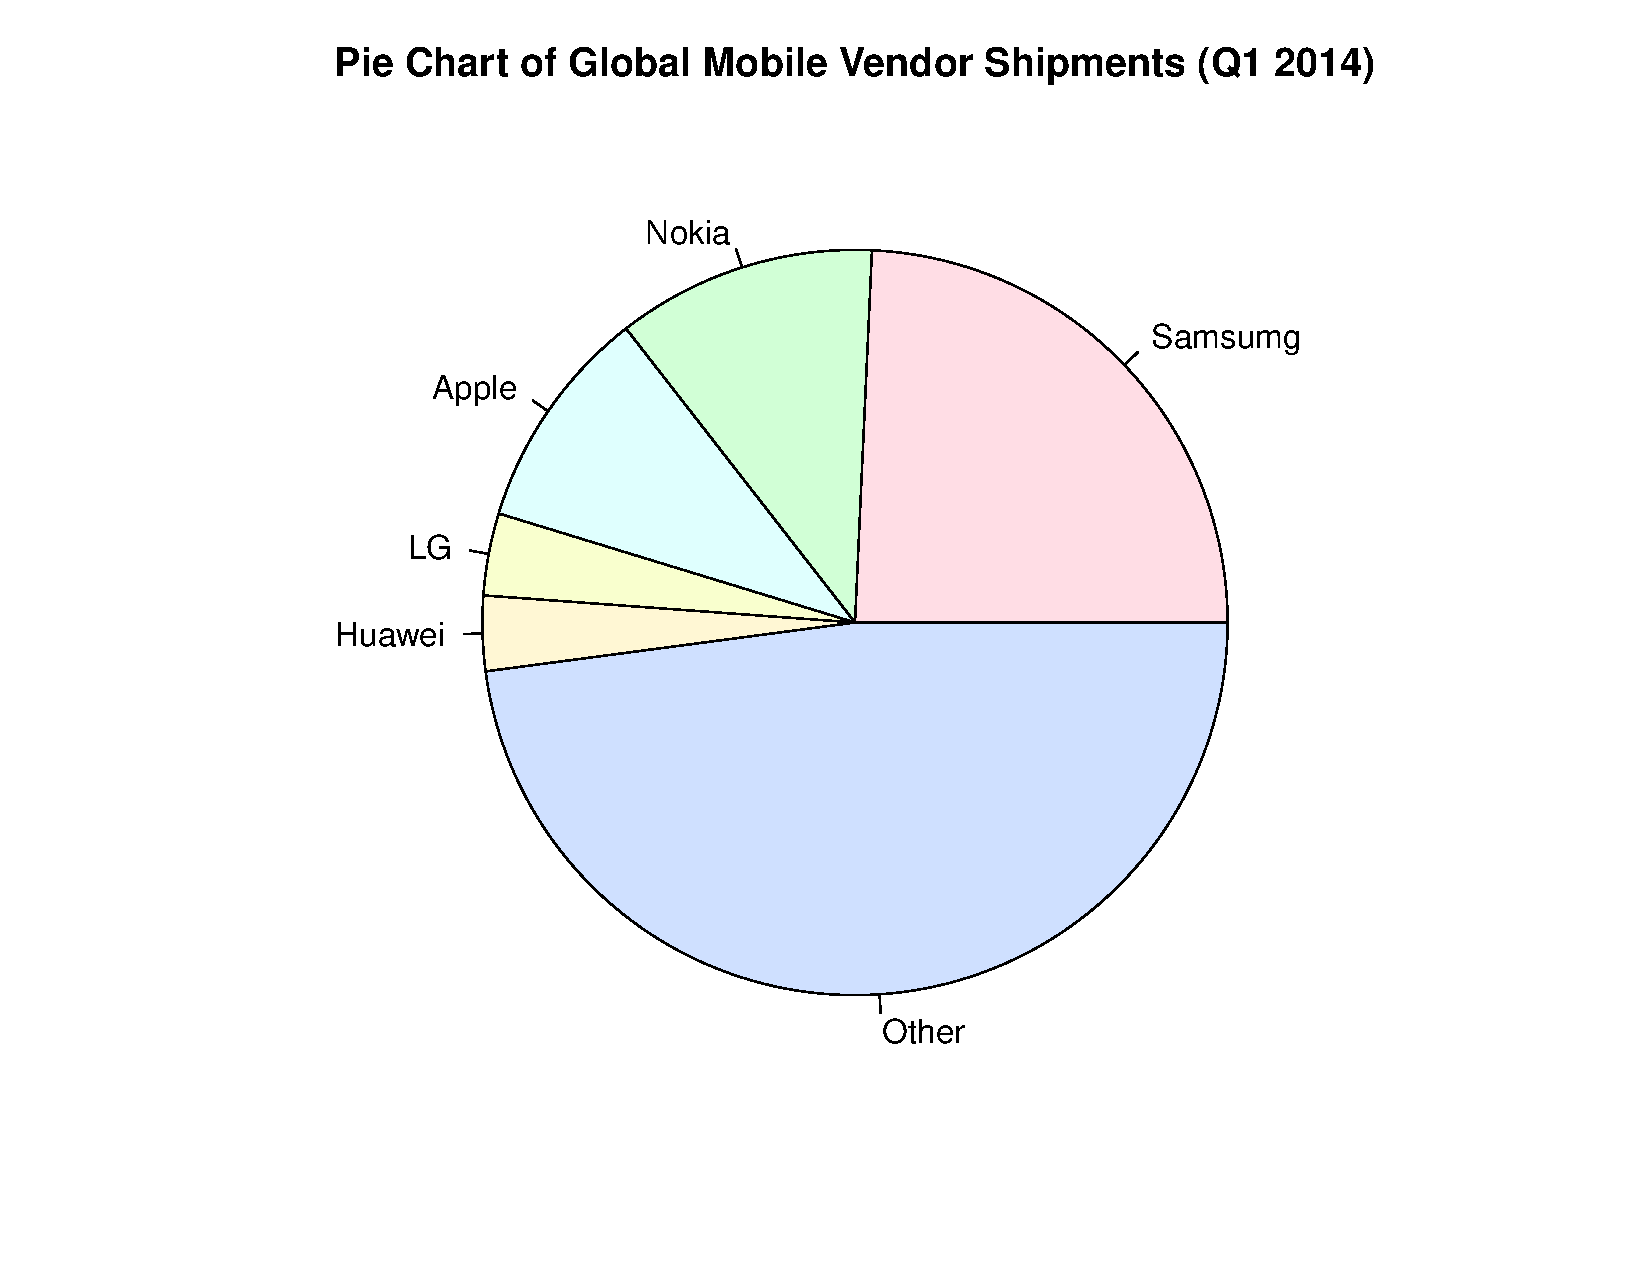
\includegraphics[scale=0.21]{pie_chart_3.pdf} };
	\node at (-3.0, 0) { 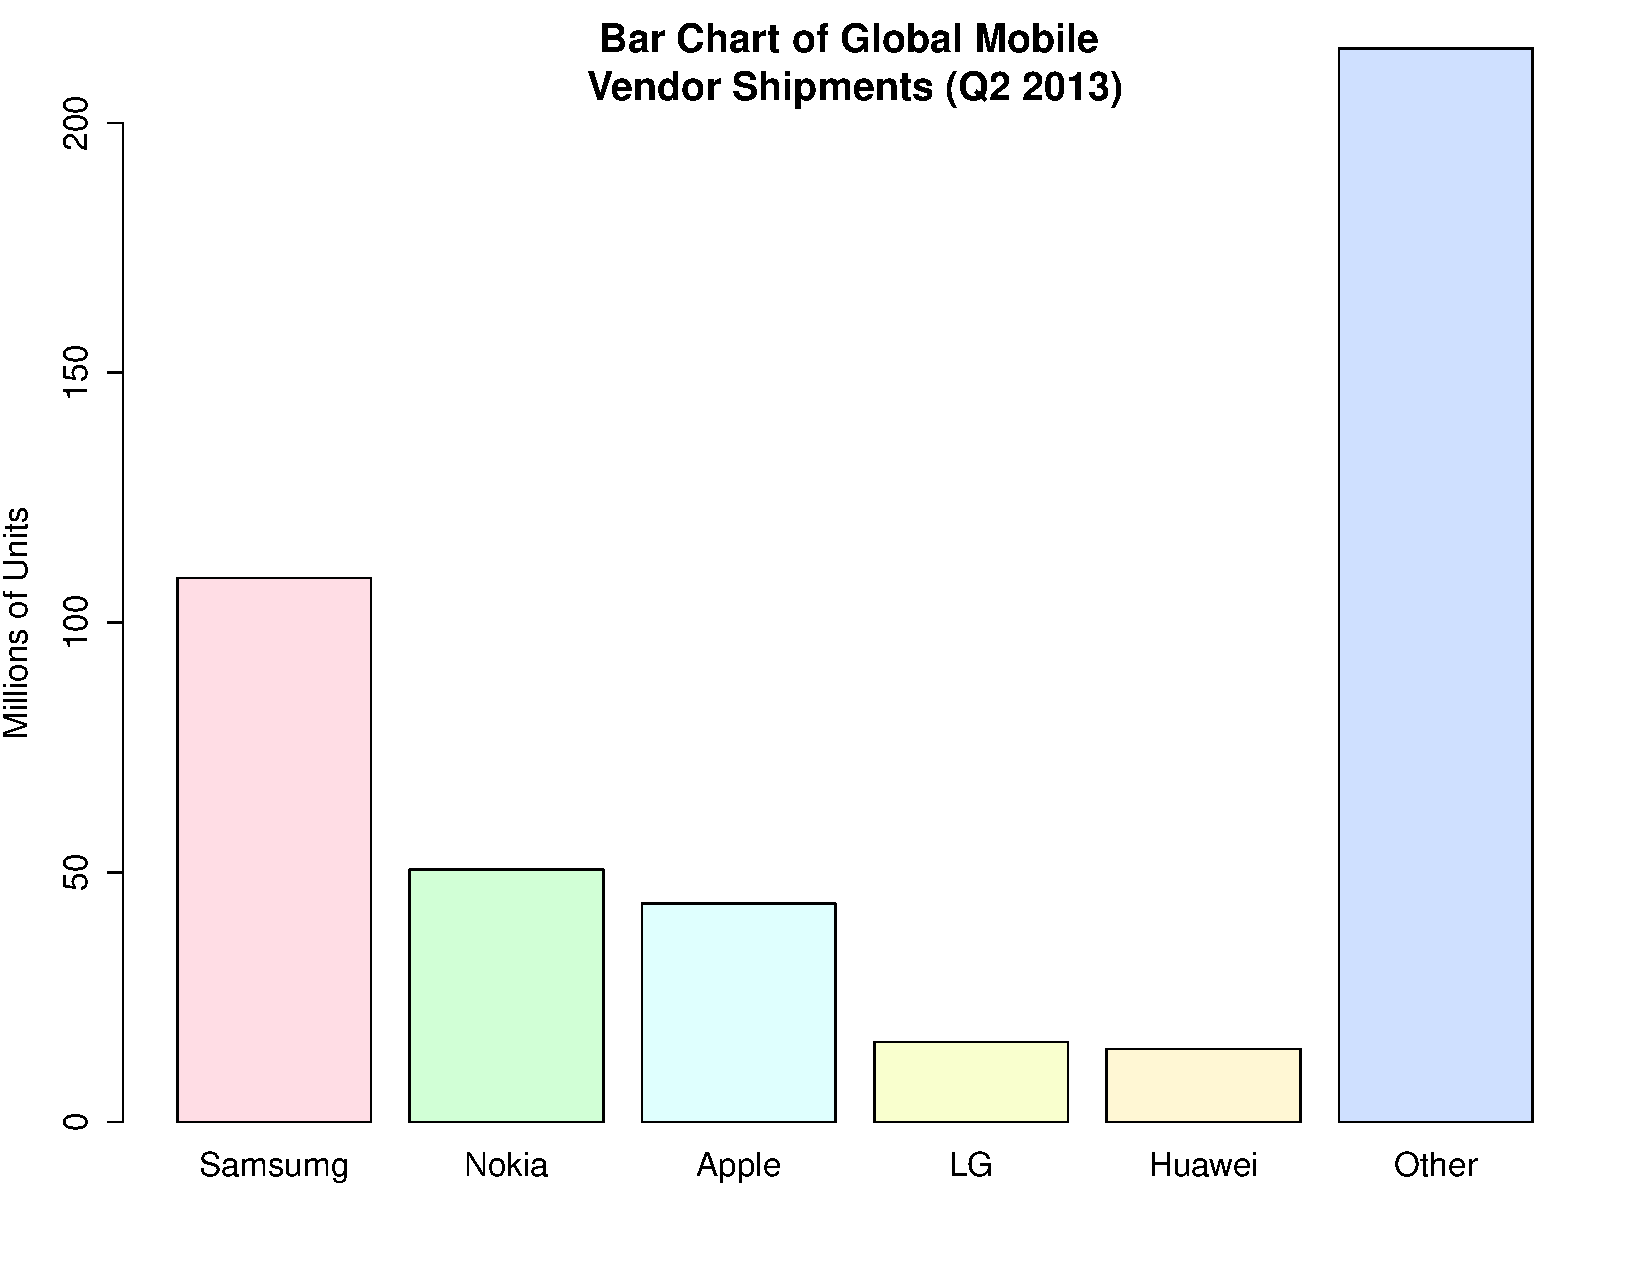
\includegraphics[scale=0.195]{bar_chart_3.pdf} };
\end{tikzpicture}
\end{center}


\tiny

\vspace{-5.50cm}
\begin{center}
\begin{tabular}{lr}
Manufacturer 	& Q2 2013 Shipments 	\\
			& (Millions of units)		\\
\hline
Samsung	&	108.9	\\
Nokia	&	50.5		\\
Apple	&	43.7		\\
LG		&	16.0		\\
Huawei	&	14.6		\\
Other	&	214.9	\\
\hline
\end{tabular}
\end{center}
\vspace{-0.35cm}
\hspace{3.4cm} \tiny{Source: IDC Worldwide Mobile Phone Tracker,2014}	




%\begin{tabular}{cc}
%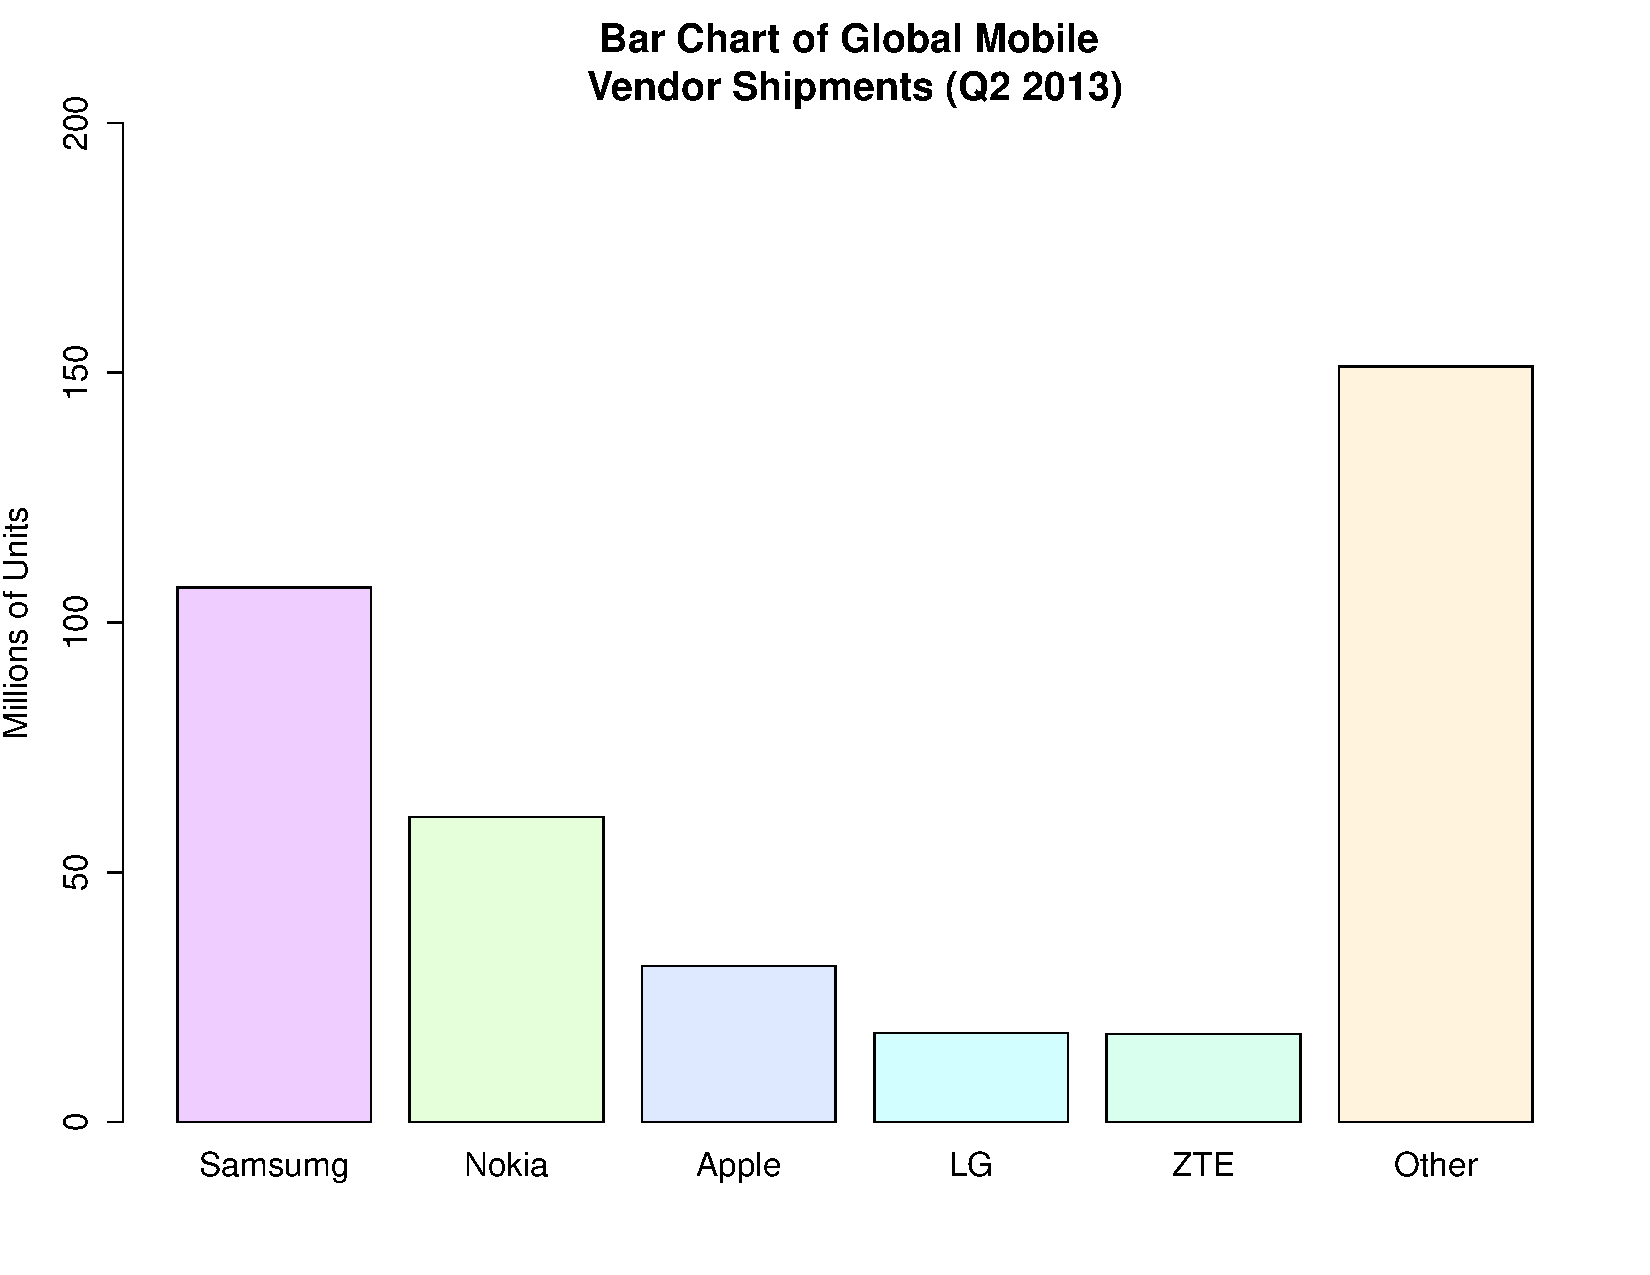
\includegraphics[scale=0.20]{bar_chart.pdf} & 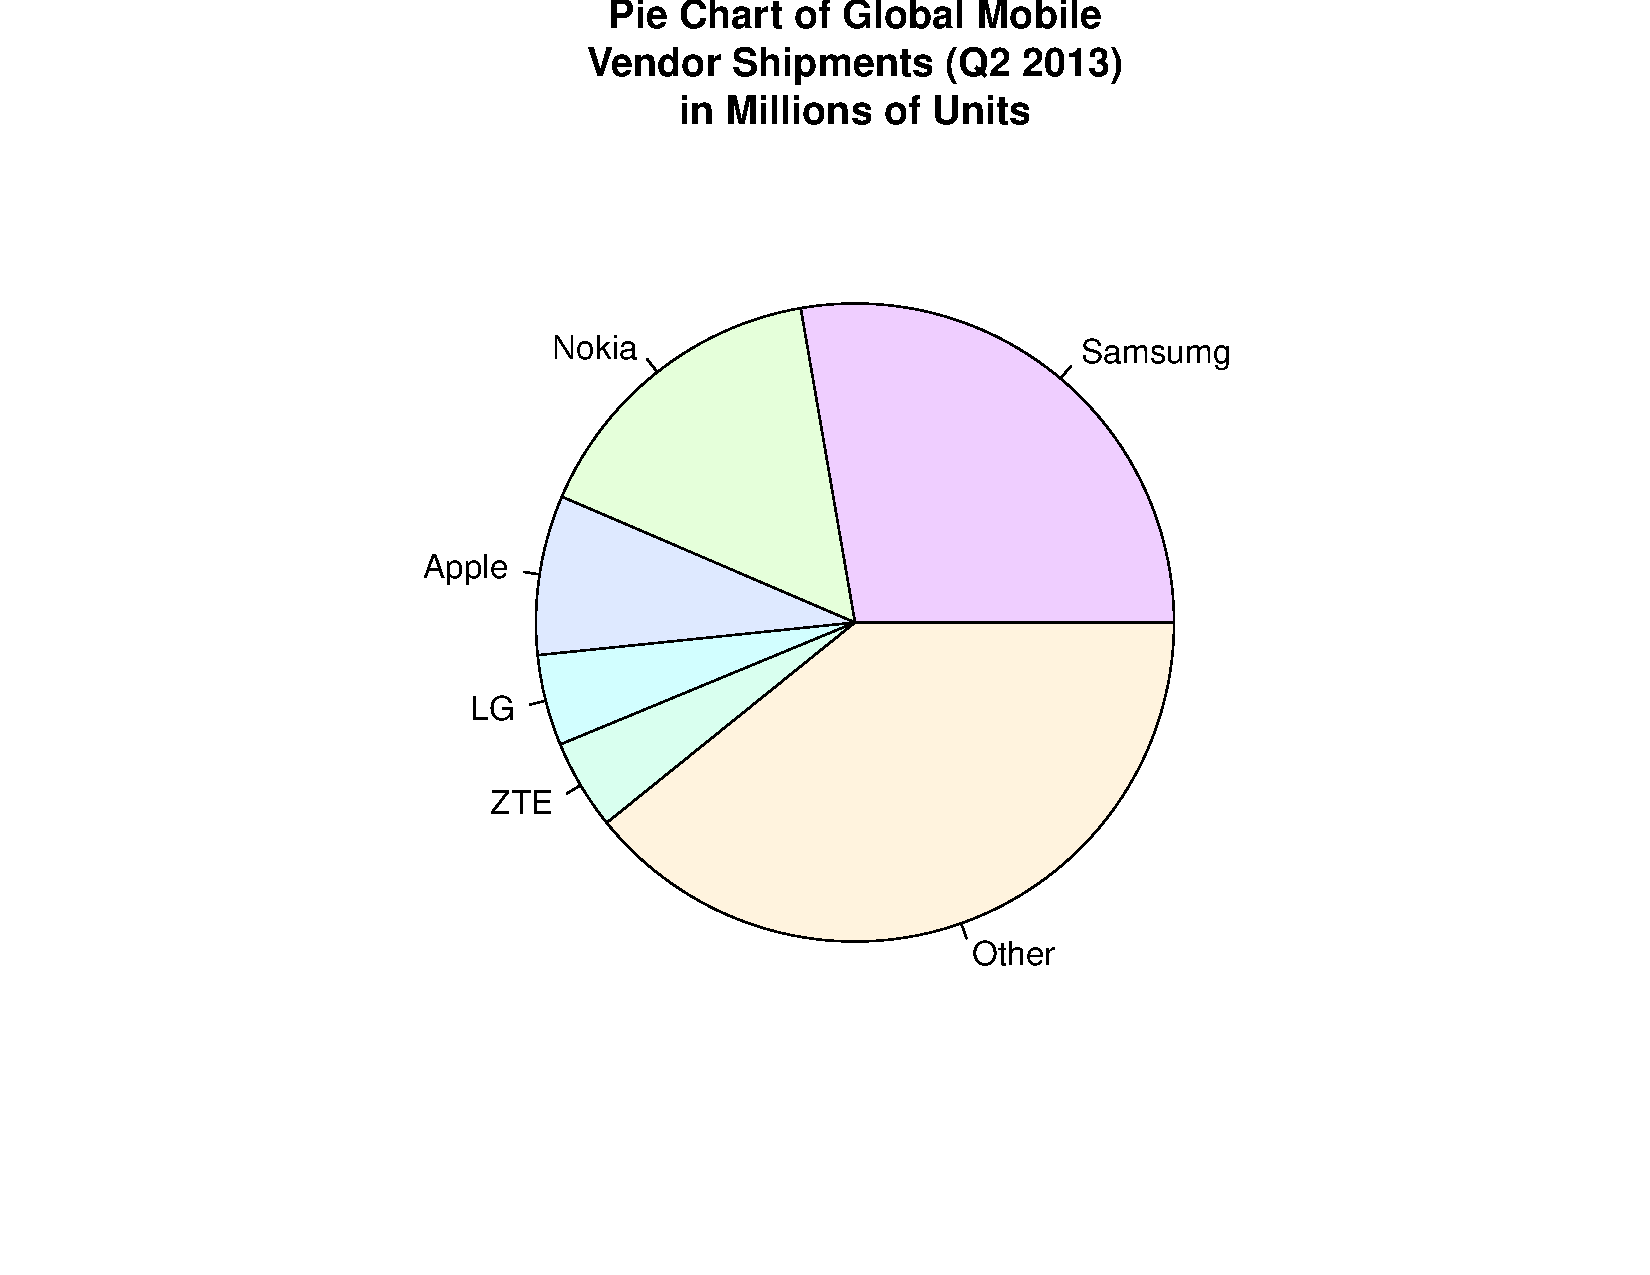
\includegraphics[scale=0.30]{pie_chart.pdf}
%\end{tabular}


\end{frame}




%\subsection*{Histograms}

\begin{frame}[t]
\frametitle{Histograms}

\begin{itemize}
\justifying
\item	A \alert{histogram} is a graphical way to represent (quantitative) data.\\
\hfill\\
\item	Similar to a bar chart but only for quantitative data.\\
\hfill\\
%\item	Suppose we had a lot of data.
\item	We make \alert{class intervals} (of equal or varying width) which will contain our data of interest.\\
\hfill\\
\item	We then count the \alert{frequency} at which we observe data falling into one of these class intervals and construct a \alert{frequency table}.\\
\end{itemize}

\end{frame}



%\subsection*{Histograms}

\begin{frame}[t]
\frametitle{Histograms Ctd...}

\vspace{-0.25cm}

\begin{itemize}
\justifying
\item	A \alert{frequency table} contains 
	\begin{itemize}
	\item	\alert{Frequencies} which are the counts that fall into an interval.	\\
	\item	\alert{Relative frequencies} which are the \alert{percentage} of counts that fall into an interval.	\\
	\end{itemize}
%\hfill\\
\hfill\\
\item	In a \alert{Frequency Histogram}, the class intervals become the width of the bars of the histogram and the \alert{frequency} will become the heights.\\
\hfill\\
\item In a \alert{Relative Frequency Histogram}, the class intervals become the width of the bars of the histogram and the \alert{relative frequencies} will become the heights.\\
\end{itemize}
\hfill\\
\vspace{0.1cm}
\justifying
\textbf{Note:} When we use the term ``histogram'' on its own, we usually refer to a frequency histogram.

\end{frame}




%\subsection*{Histograms}

% \rotatebox{90}{\Kutline}

\begin{frame} %[t]
\frametitle{Histograms Ctd...}
General form of a \alert{frequency table}
\vspace{-0.25cm}
\footnotesize
\begin{center}
\begin{tabular}{c c c c l l}
Class			&	Freq.		&	Relative			&	&	Cumulative				&	Cumulative	\\
Interval			&			&	Freq.				&  	&	Freq.						&	Relative Freq.	\\
\hline
$[a_{1}, b_{1})$		&	$f_{1}$	&	$r_{1} = f_{1} / F$	& 	&	$f_{1}$					&	$r_{1}$\\
$[a_{2}, b_{2})$		&	$f_{2}$	&	$r_{2} = f_{2} / F$	&  	&	$f_{1} + f_{2}$				&	$r_{1}+r_{2}$\\
$[a_{3}, b_{3})$		&	$f_{3}$	&	$r_{3} = f_{3} / F$	& 	&	$f_{1} + f_{2} + f_{3}$		&	$r_{1}+r_{2}+r_{3}$\\
\vdots			&	\vdots	&	\vdots			&  	&	\hspace{0.75cm} \vdots		&	\hspace{0.75cm} \vdots\\
$[a_{m}, b_{m}]$	&	$f_{m}$	&	$r_{m} = f_{m} / F$	& 	&	$f_{1} + \ldots + f_{m} = F$	&	$r_{1} + \ldots + r_{m} = 1$\\
\hline
				&	$F = \displaystyle\sum_{i=1}^{m} f_{i}$ & 1 \\
\end{tabular}
\end{center}

\begin{tikzpicture}[overlay]
\draw [dashed] (5.32,0.30) -- (5.32,4.375);
\end{tikzpicture}

It may look overwhelming, but we will do an example.

\end{frame}




%\subsection*{Histograms}

\begin{frame} %[t]
\frametitle{Example}

\justifying
Suppose we have the following set of 30 observations which represents manufacturing times (in days) for mining equipment:
\hfill\\

\begin{center}
\begin{tabular}{r r r r r r r r r r  }
53	& 	51	&	92	&	53	&	77	&	78	&	77	&	76	&	53	&	40	\\
45	&	60	&	99 	&	64 	&	44	&	93	&	64	&	45	&	53	&	26	\\
58	&	114	&	35	&	64	&	58	&	118	&	74	&	37	&	48	&	39	\\
%52	&	53	&	43	&	53	&	90	&	42	&	90	&	31	&	52	&	99	\\
%46	&	86	&	64	&	91	& 	39	&	53 	& 	54	&	111	&	19	& 	97 	\\
%44 	& 	67 	& 	88 	& 	34 	&	108 	& 	45 	& 	55	&	88	&	75 	& 	59	\\
%70 	& 	73 	& 	98 	& 	98 	& 	68 	& 	53 	& 	52 	&	102 	& 	97 	& 	61	\\
%90 	& 	83 	&	58 	& 	72 	& 	60 	& 	70 	& 	54 	& 	70 	& 	46 	& 	100	\\
\end{tabular}
\end{center}
\hfill\\
\justifying
It is hard to see any obvious patterns with just the \alert{raw data} alone.\\
\hfill\\
\justifying
Perhaps a picture will help.

\end{frame}





\begin{frame} [t]
\frametitle{Example Ctd...}

First lets sort the data (Optional but very helpful):
\hfill\\

\begin{center}
\begin{tabular}{r r r r r r r r r r  }
26	&	35	&	37	&	39	&	40	&	44	&	45	&	45	&	48	&	51	\\
53	&	53	&	53	&	53	&	58	&	58	&	60	&	64	&	64	&	64	\\
74  	&	76	&	77	&	77	&	78	&	92	&	93	&	99	&	114	&	118	\\
%31 	& 	34 	& 39 & 42 & 43 & 44 & 45 & 46 & 46 & 52	\\
%52 	& 	52 	& 53 & 53 & 53 & 53 & 54 & 54 & 55 & 58	\\
%59 	& 	60 	& 61 & 64 & 67 & 68 & 70 & 70 & 70 & 72	\\
%73 	& 	75 	& 83 & 86 & 88 & 88 & 90 & 90 & 90 & 91	\\
%97 	& 	97 	& 98 & 98 & 99 & 100  & 102 & 108 & 111 & 119	\\
\end{tabular}
\end{center}
\hfill\\
After sorting, the following class intervals appear \alert{intuitively ``nice''}: 
\hfill\\

\begin{center}
\begin{tabular}{l c r}
Interval	& &	Mathematical	\\
		& &	representation	\\
\hline
20 to 39		& &	$[20,40)$	\\
40 to 59		& &	$[40,60)$ 	\\
60 to 79		& &	$[60,80)$	\\
80 to 99		& &	$[80,100)$	\\
100 to 120	& &	$[100,120]$ 	\\
\hline
\end{tabular}
\end{center}
%$[30,40)$   \\
%$[40,50)$   \\
%$[50,60)$   \\
%$[60,70)$   \\
%$[70,80)$   \\
%$[80,90)$  \\
%$[90,100)$ 	\\
%$[100,110)$ 	\\
%$[110,120]$ 

\end{frame}







\begin{frame} [t]
\frametitle{Example Ctd...}

\vspace{-0.5cm}

\begin{center}
\begin{tabular}{r r r r r r r r r r  }
26	&	35	&	37	&	39	&	40	&	44	&	45	&	45	&	48	&	51	\\
53	&	53	&	53	&	53	&	58	&	58	&	60	&	64	&	64	&	64	\\
74  	&	76	&	77	&	77	&	78	&	92	&	93	&	99	&	114	&	118	\\
%31 	& 	34 	& 39 & 42 & 43 & 44 & 45 & 46 & 46 & 52	\\
%52 	& 	52 	& 53 & 53 & 53 & 53 & 54 & 54 & 55 & 58	\\
%59 	& 	60 	& 61 & 64 & 67 & 68 & 70 & 70 & 70 & 72	\\
%73 	& 	75 	& 83 & 86 & 88 & 88 & 90 & 90 & 90 & 91	\\
%97 	& 	97 	& 98 & 98 & 99 & 100  & 102 & 108 & 111 & 119	\\
\end{tabular}
\end{center}
\hfill\\
Complete the frequency table: 
\hfill\\


\scriptsize

\begin{center}
\begin{tabular}{r c l l l}
Class \hspace{0.25cm}	&	~Freq.~	&	\hspace{0.30cm} Relative \hspace{0.30cm}	&	\hspace{0.30cm} Cumulative \hspace{0.30cm}	&	\hspace{0.30cm} Cumulative	\\
Interval			 	&			&	\hspace{0.30cm} Freq.					&	\hspace{0.30cm} Freq.					&	\hspace{0.30cm} Relative Freq. \hspace{0.30cm} \\
\hline
$[20,40)$			&	\\
\hfill\\
$[40,60)$ 			&	\\
\hfill\\
$[60,80)$			&	\\
\hfill\\
$[80,100)$		&	\\
\hfill\\
$[100,120]$ 		&	\\
\hline
\end{tabular}
\end{center}

\end{frame}

 
 
 
 









\begin{frame} [t]
\frametitle{Example Ctd...}

\tiny{

\vspace{-0.75cm}
\scriptsize
\begin{center}
\begin{tabular}{r r l r l}
Class \hspace{0.25cm}	&	\quad  Freq.	&	\quad Relative 		&	\quad Cumulative 		& \quad Cumulative		\\
Interval			 	&				&	\quad Freq.		&	Freq. \hspace{0.60cm}	& \quad Relative Freq.	\\
\hline
$[20,40)$				&	4	\quad       	&	\quad 0.13333333	&	4	\hspace{0.25cm}	& \quad 0.13333333	\\
$[40,60)$ 				&	12     \quad	&	\quad 0.40		&	16	\hspace{0.25cm}	& \quad 0.53333333 \\
$[60,80)$				&	9	\quad	&	\quad 0.30		&	25	\hspace{0.25cm}	& \quad 0.83333333 \\
$[80,100)$			&	3	\quad	&	\quad 0.10		&	28	\hspace{0.25cm}	& \quad 0.93333333	\\
$[100,120]$ 			&	2	\quad	&	\quad 0.06666667	&	30	\hspace{0.25cm}	& \quad 1	\\
\hline
					&	30	\quad	&	\quad 1
\end{tabular}
\end{center}
}

\vspace{-1.0cm}

\begin{center}
%\begin{tabular}{cc}
%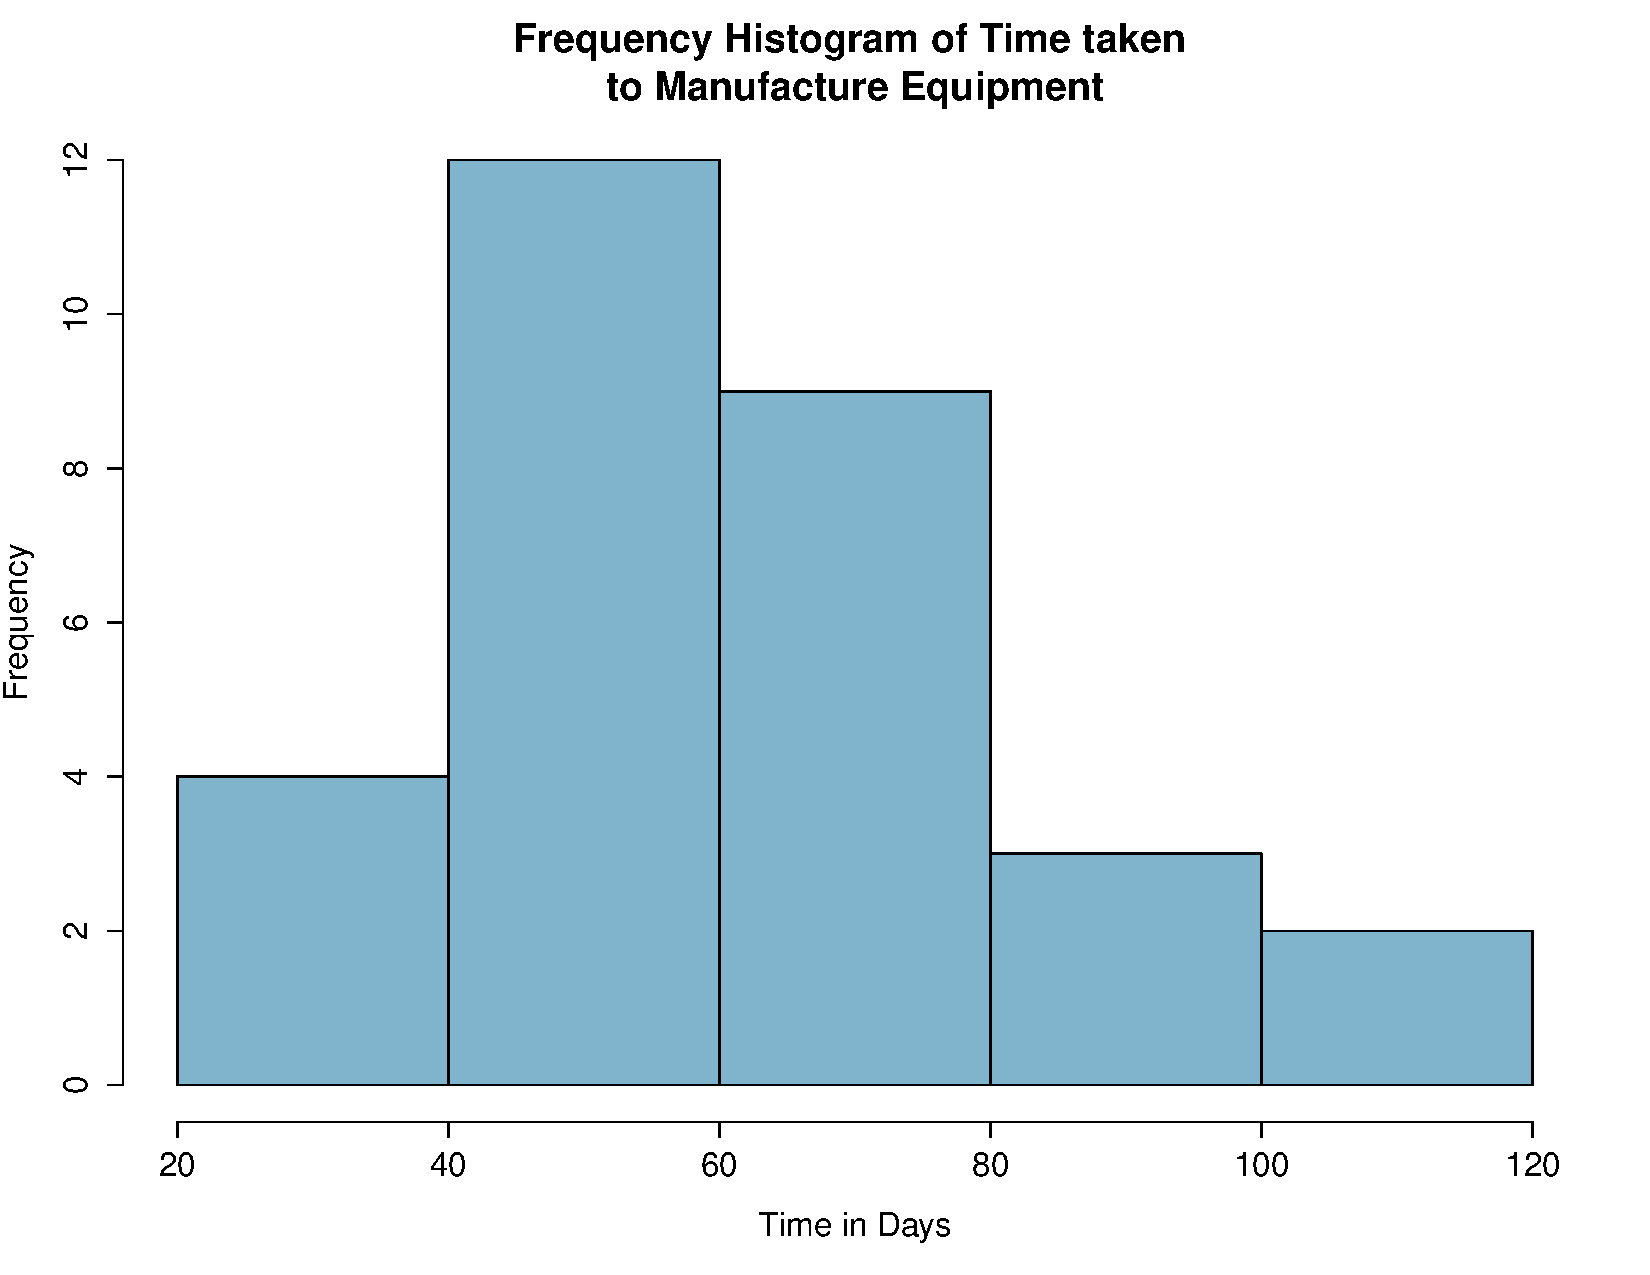
\includegraphics[scale=0.20]{freq_hist.pdf}	&	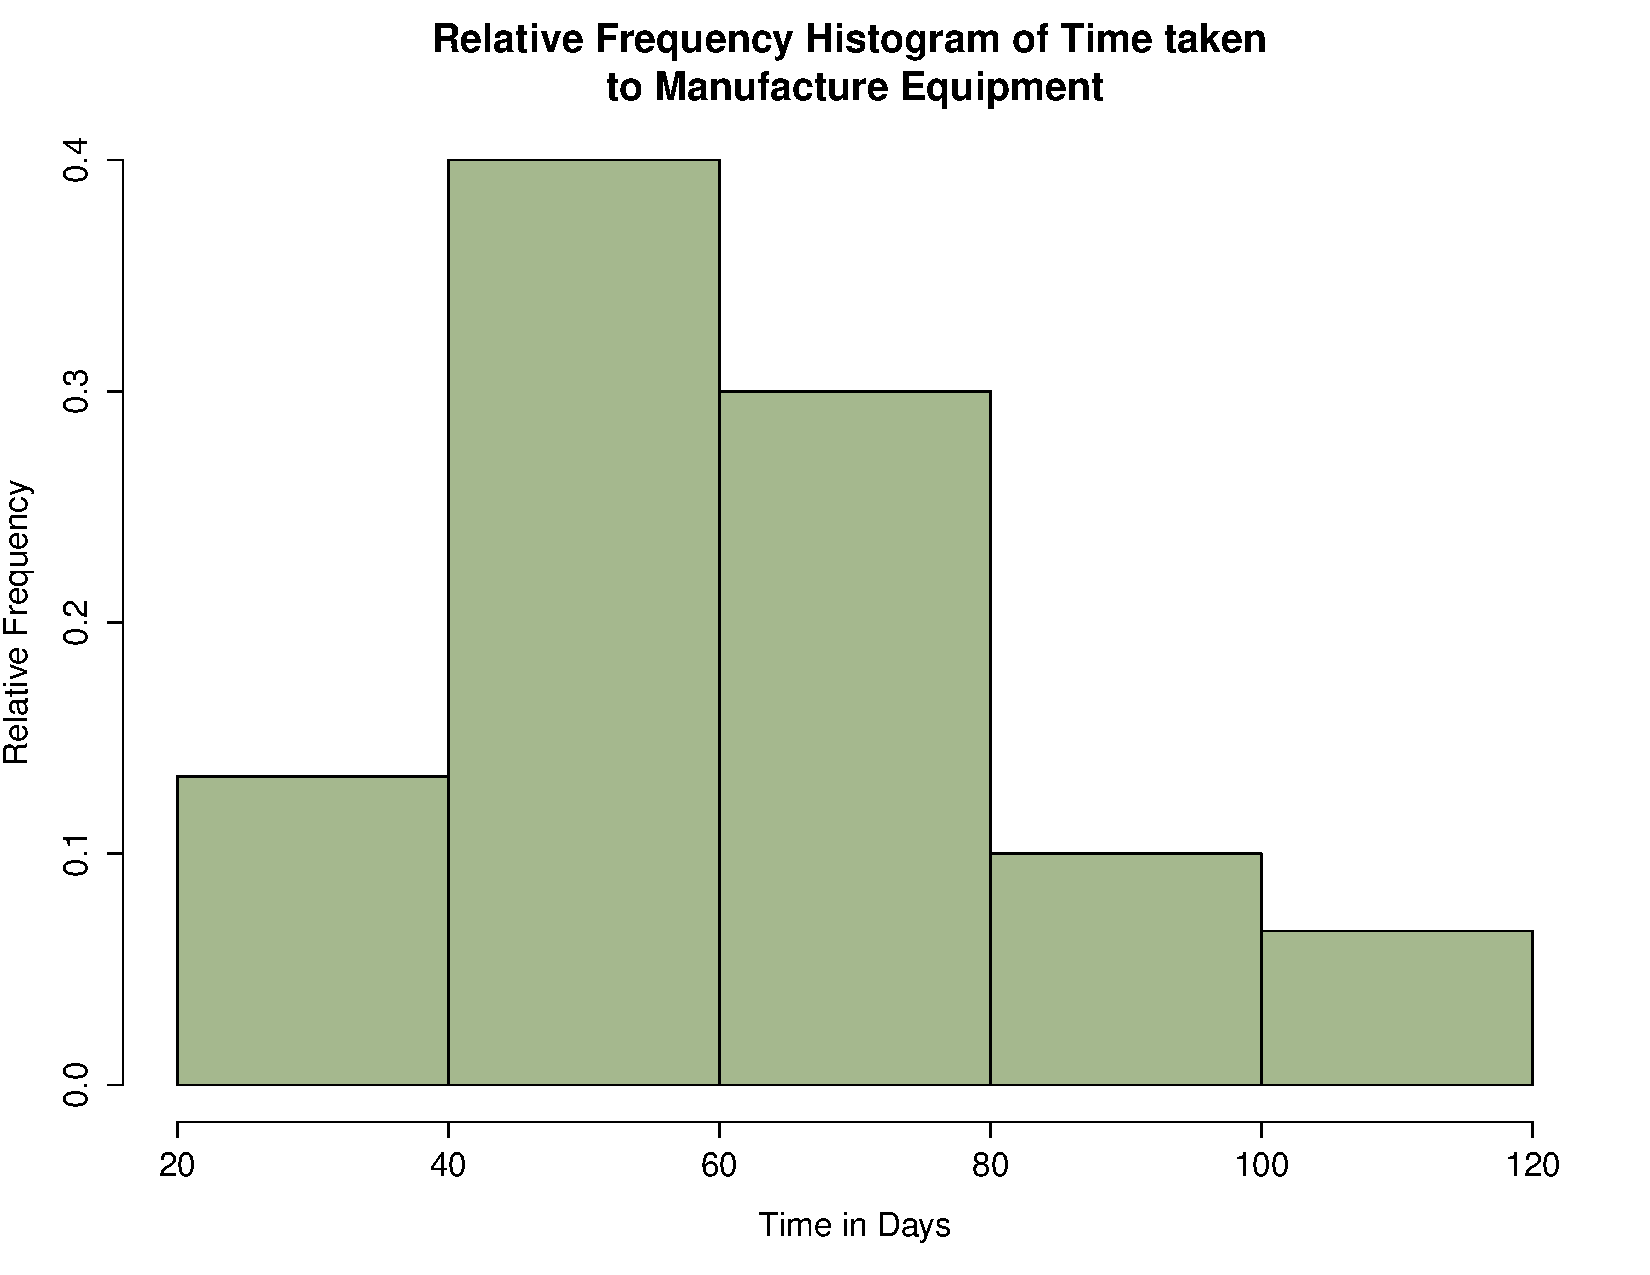
\includegraphics[scale=0.20]{rel_freq_hist.pdf}
%\end{tabular}
\begin{tikzpicture}[overlay]
	\node at (-2.50, -2.30) { 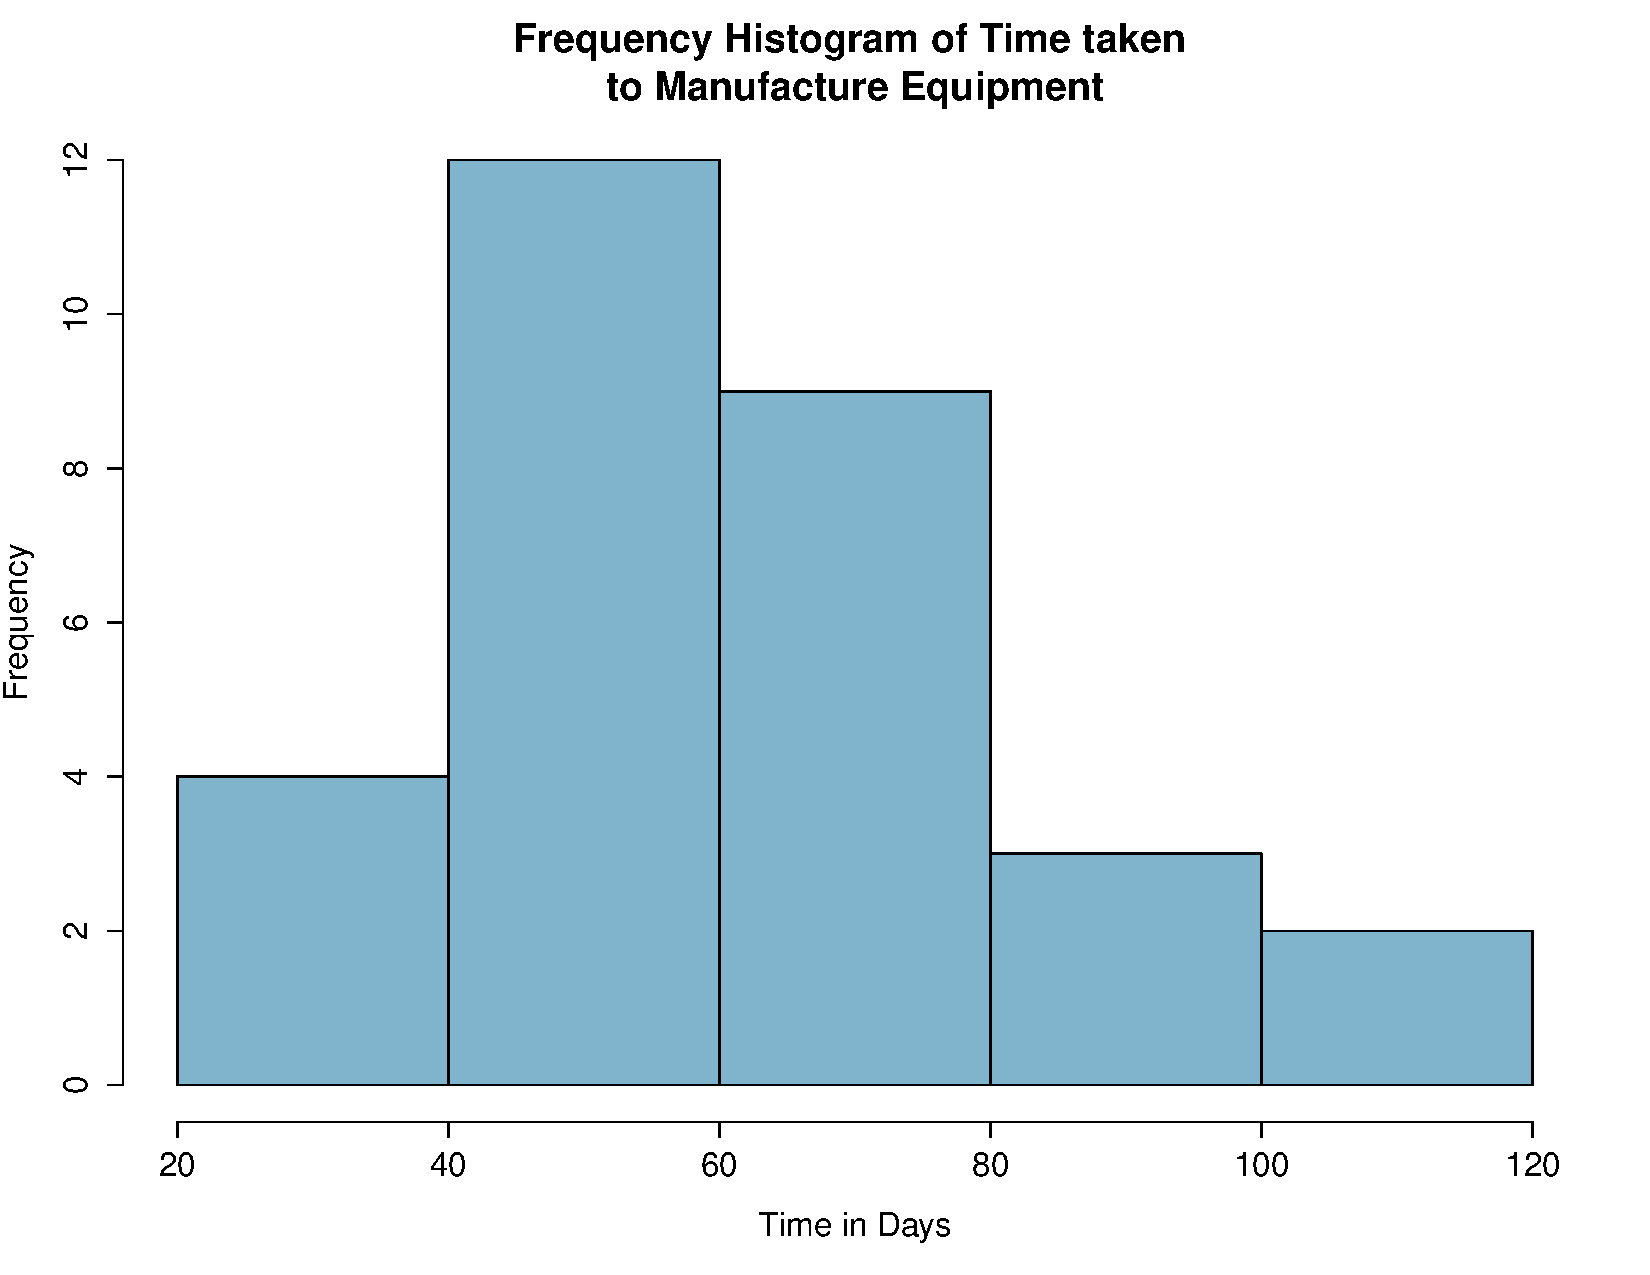
\includegraphics[scale=0.175]{freq_hist.pdf} };
	\node at (3.0, -2.30) { 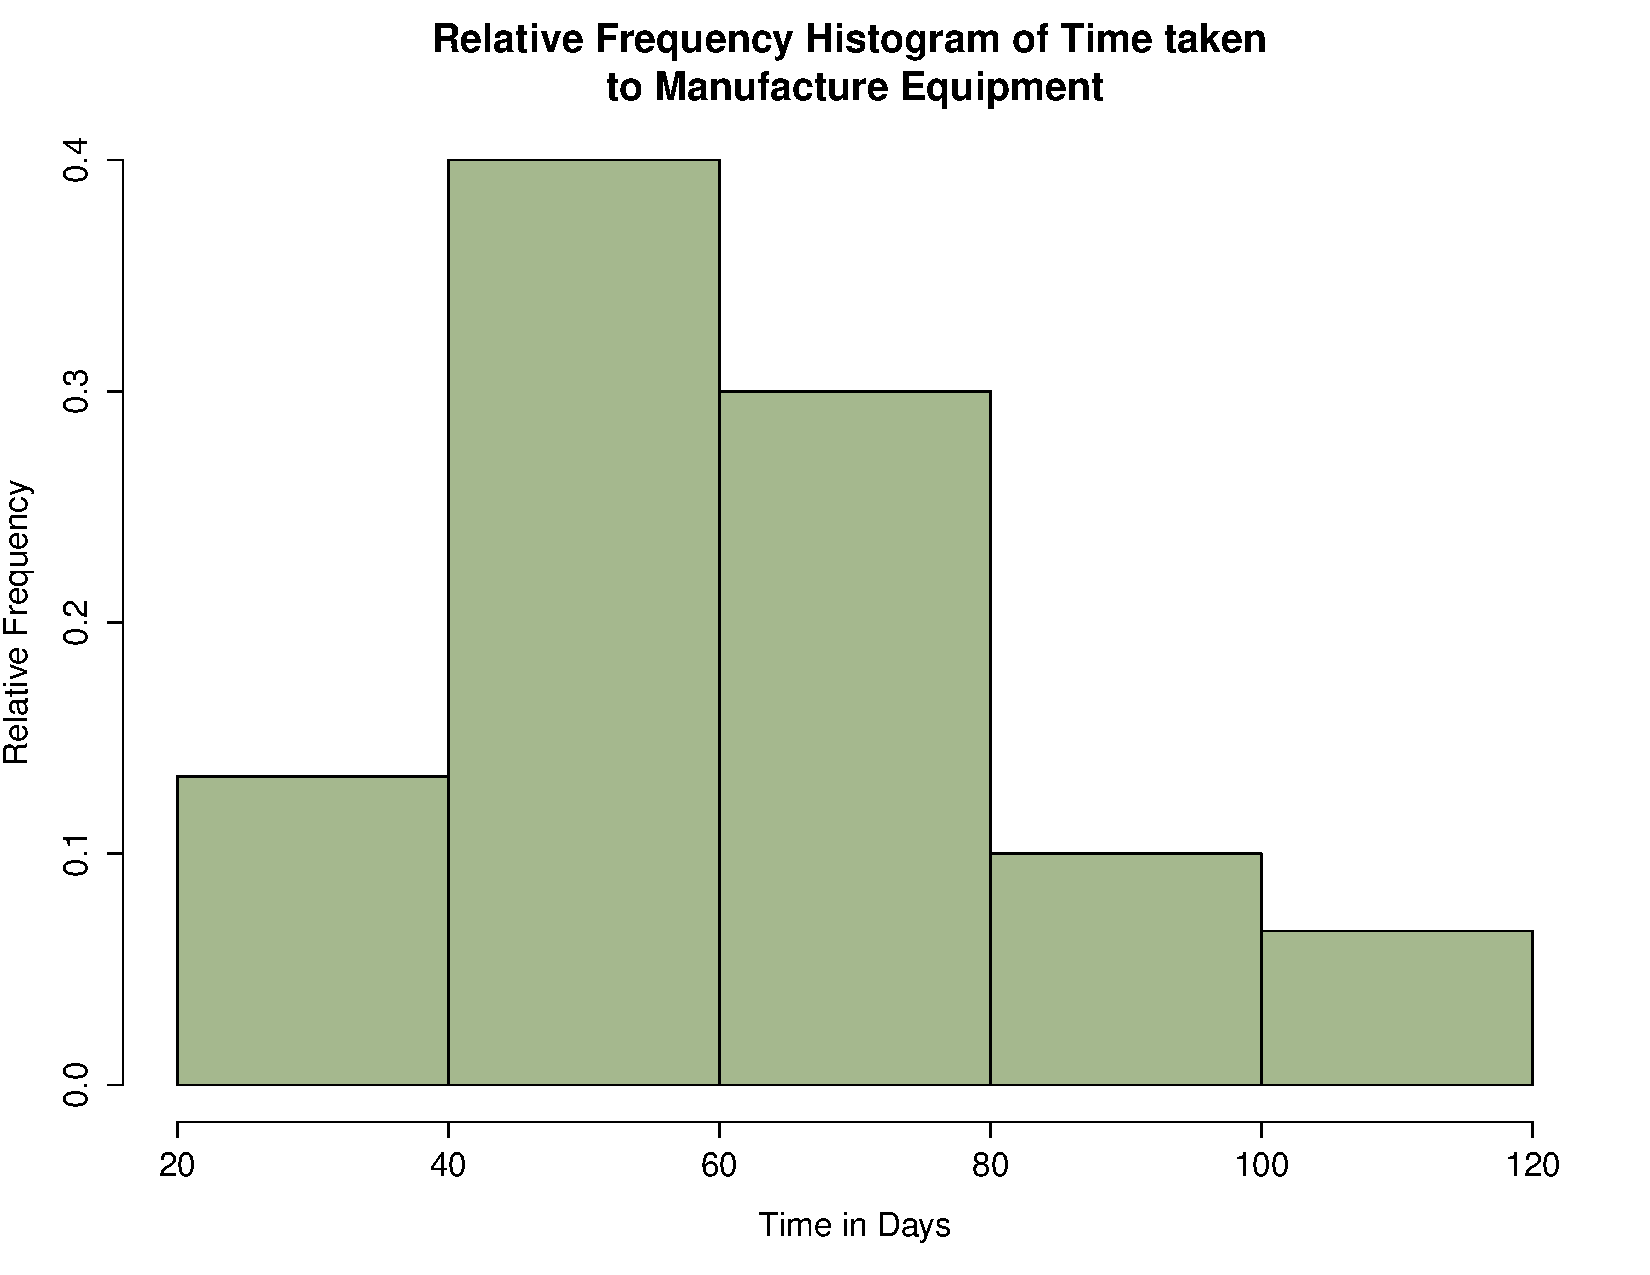
\includegraphics[scale=0.175]{rel_freq_hist.pdf} };
\end{tikzpicture}
\end{center}

\end{frame}




%\subsection*{Estimating the Mean using a Histogram}

\begin{frame}%[t]
\frametitle{Estimating the Mean using a Histogram}

\begin{itemize}
\justifying
\item	We \underline{estimate} the mean of a histogram using


\begin{equation*}
Estimated ~ mean = \frac{ \sum (mid point ~  of ~ class ~ interval) \cdot (frequency) }{total}
\end{equation*}

\hfill\\
\item	Note that this estimation assumes a uniform spread of the date in each class interval.
\end{itemize}

\end{frame}



%\subsection*{Example}

\begin{frame}[t]
\frametitle{Example}

\vspace{-1.0cm}

\small
Estimate the mean of the following histogram

\vspace*{-0.4cm}
\begin{center}
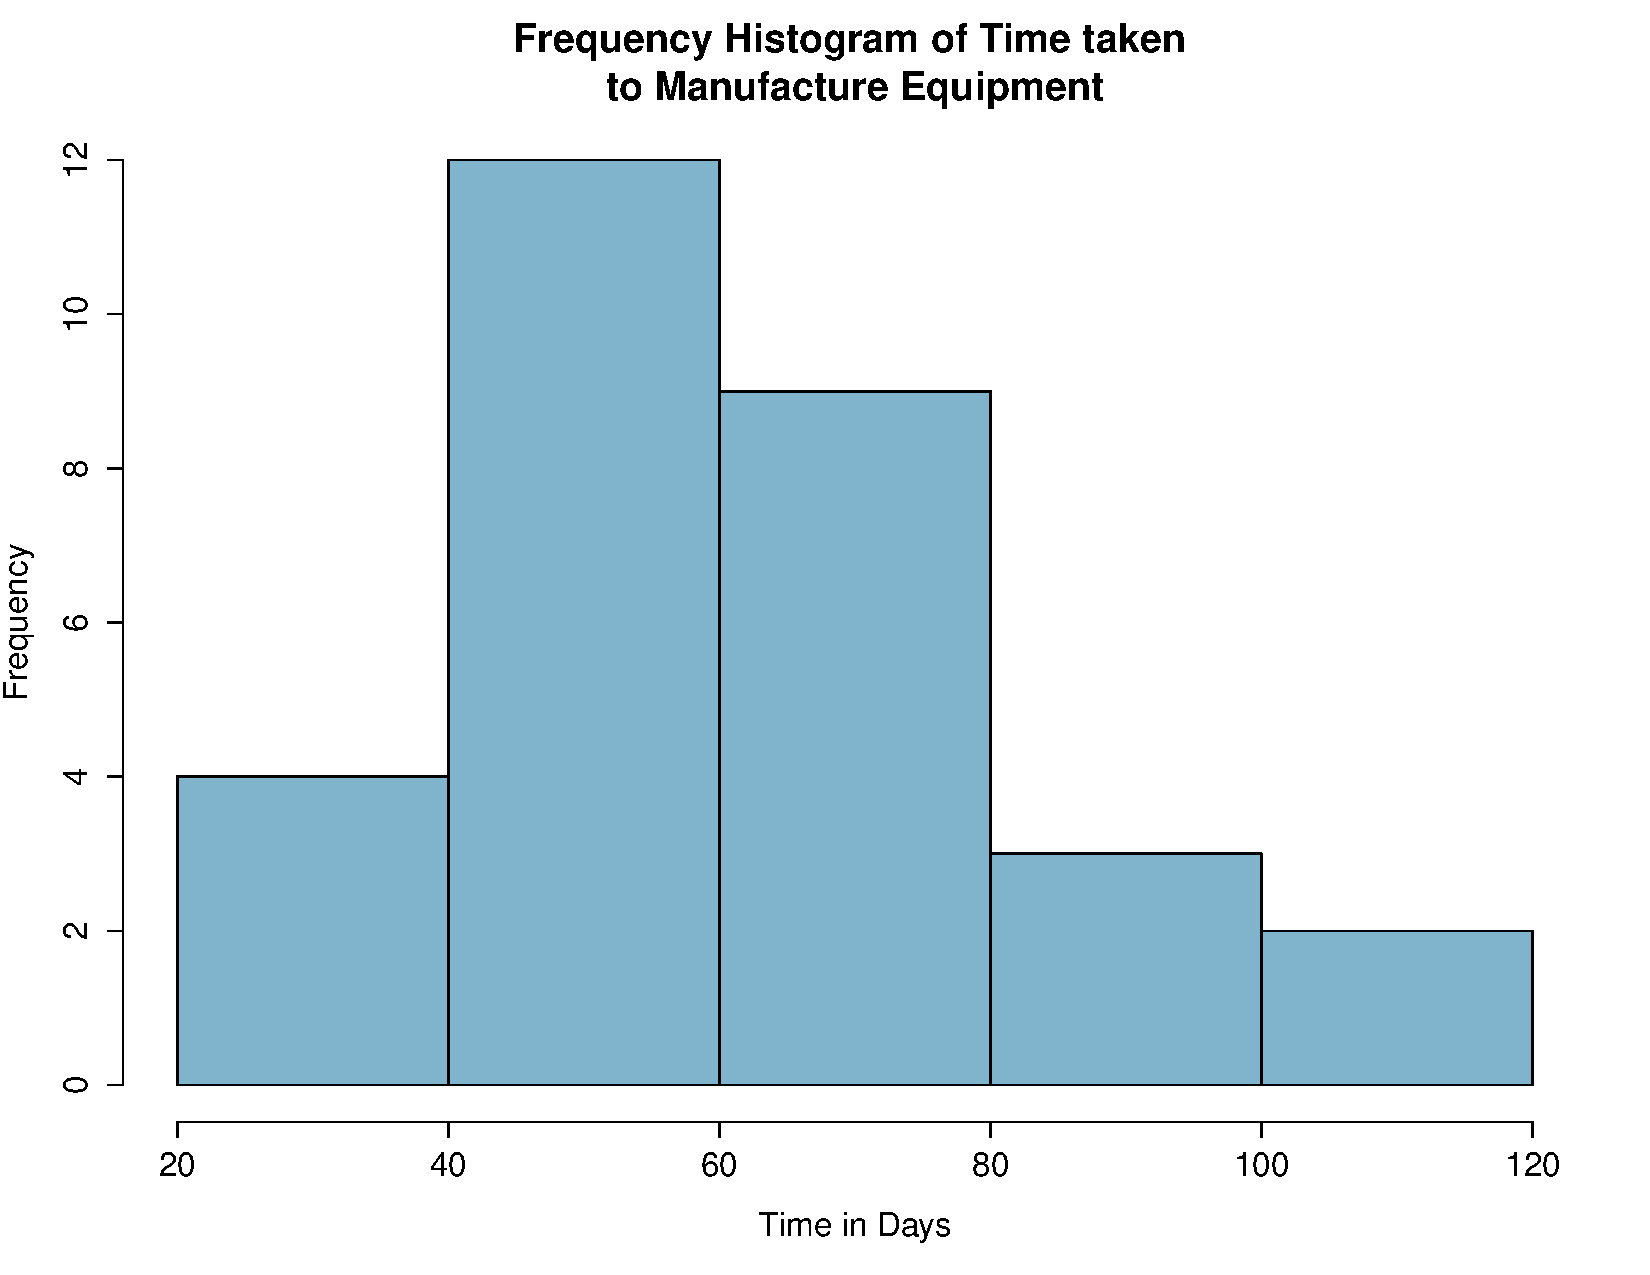
\includegraphics[scale=0.18]{freq_hist.pdf} 
\end{center}

\end{frame}



%\subsection*{Skewness}

\begin{frame}
\frametitle{Skewness}

\vspace{-0.5cm}

\begin{itemize}
\justifying
\item	\alert{Skewness} is a measure of how much a distribution leans towards a particular side or whether it is symmetric.\\
	\hfill\\
	\begin{tabular}{lcl}
	\justifying
	\alert{Symmetric}		& : 	&	\makebox[5.65cm][s]{Most observations are concentrated}	\\
						&	&	\makebox[5.65cm][s]{around the mean and tail off fairly}		\\
						&	&	\makebox[5.25cm][s]{evenly on both sides of the mean.}		\\
	\hfill\\
	\alert{Right skewed}		& :	&	\makebox[5.65cm][s]{We observe a tail to the right side} 	\\
		(Positively skewed)	&	&	\makebox[5.65cm][s]{of the mean. More observations are}	\\
						&	&	\makebox[5.25cm][s]{concentrated on smaller values.}	\\
	\hfill\\
	\alert{Left skewed}		& :	&	\makebox[5.65cm][s]{We observe a tail to the left side} 	\\
		(Negatively skewed)	&	&	\makebox[5.65cm][s]{of the mean. More observations are}	\\
						&	&	\makebox[5.25cm][s]{concentrated on larger values.}		\\
	
	\end{tabular}
\hfill\\
\end{itemize}

\end{frame}




%\subsection*{Skewness}

\begin{frame}
\frametitle{Skewness Ctd...}

\begin{itemize}
\justifying
\item	We can usually determine the skewness of a distribution by visually observing a histogram.\\
\hfill\\
\item	By noting skewness, we get even more information about our data. \\
\hfill\\
\item	Note however that we may not always be able to tell the skewness by visually observing a histogram.
\end{itemize}

\end{frame}




%\subsection*{Skewness}

\begin{frame}
\frametitle{Skewness Ctd...}

\vspace{-0.50cm}
\underline{Symmetric}

% Red = Mean
% Blue = Median
\begin{picture}(200,200)
\put(0,0){ 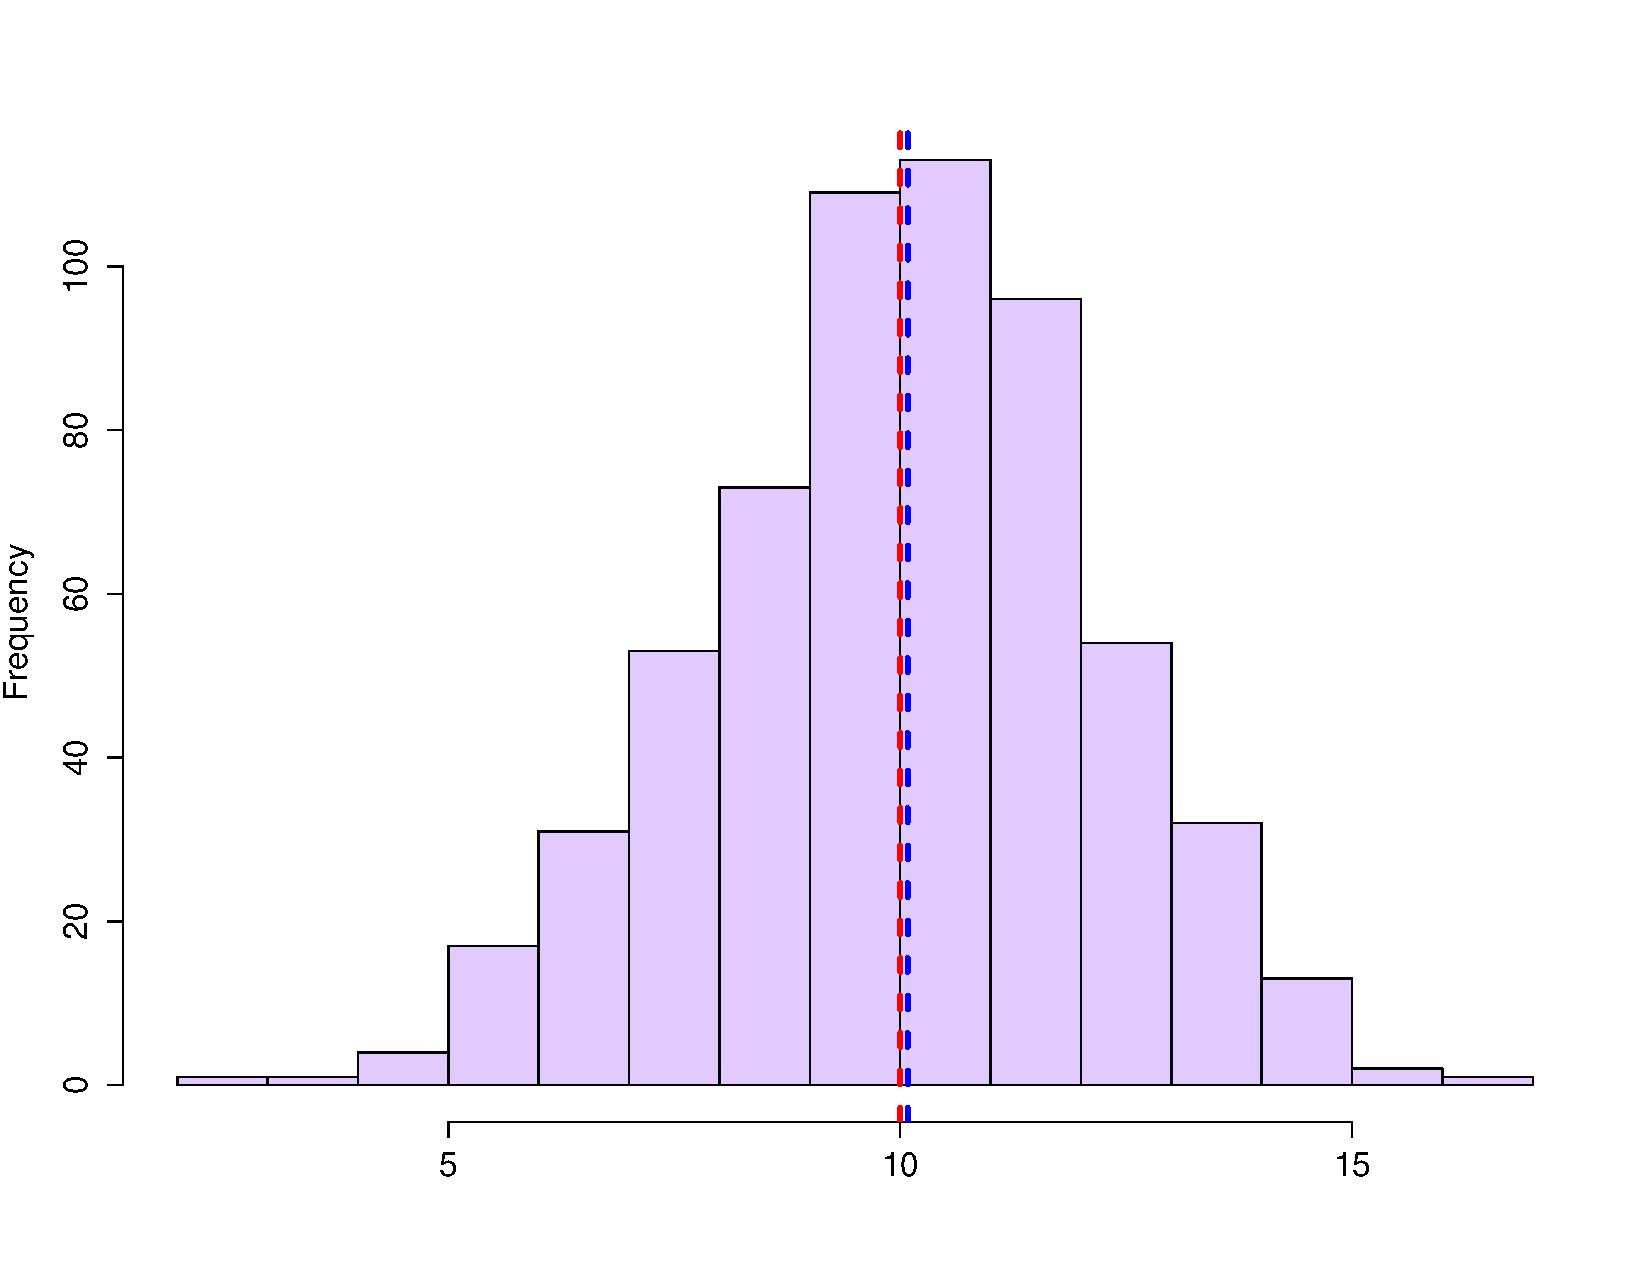
\includegraphics[scale=0.325]{symm.pdf} } 
\put(225,150){\hbox{mean	\quad\quad	median}}
\end{picture}

\end{frame}




%\subsection*{Skewness}

\begin{frame}
\frametitle{Skewness Ctd...}

\vspace{-0.50cm}
\underline{Skewed to the Right}

\begin{picture}(200,200)
\put(0,0){ 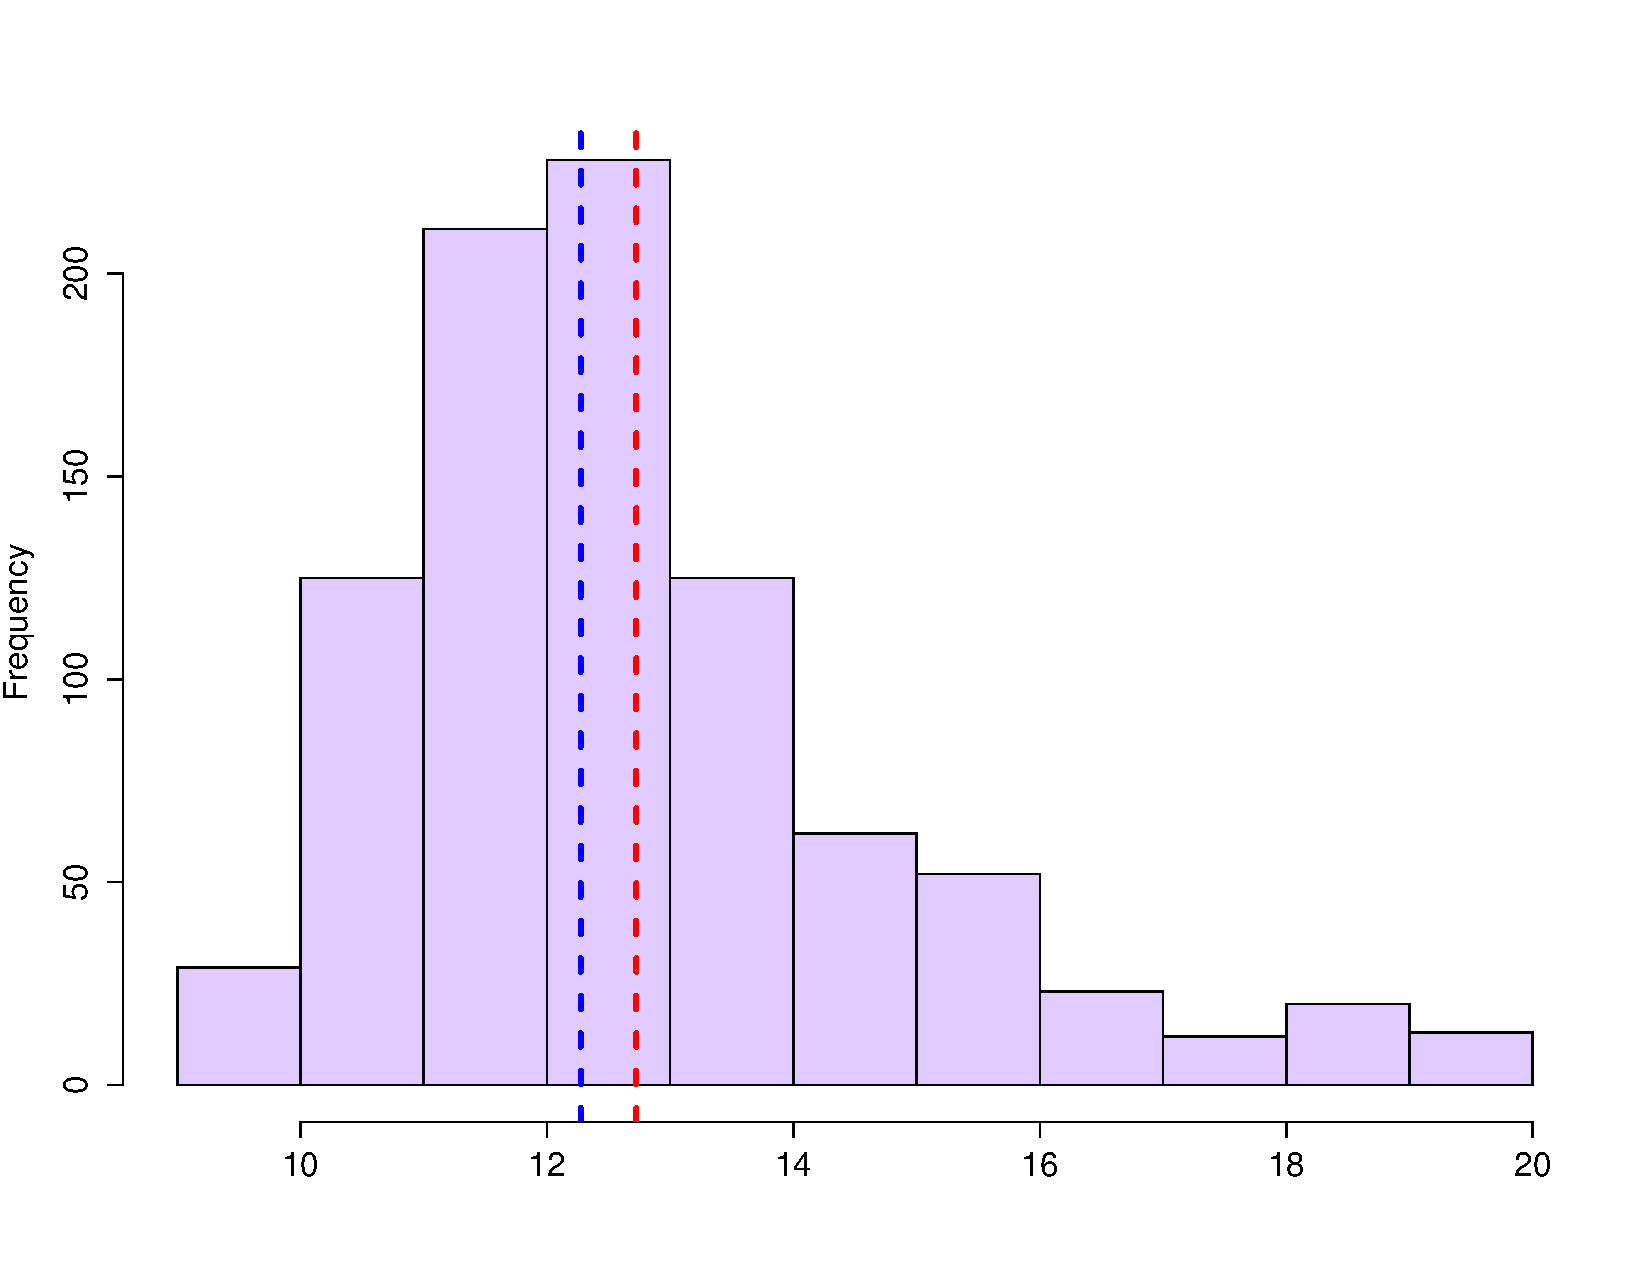
\includegraphics[scale=0.325]{skew_right.pdf} } 
\put(225,150){\hbox{mean	\quad\quad	median}}
\end{picture}


\end{frame}



\subsection*{Skewness}

\begin{frame}
\frametitle{Skewness Ctd...}

\vspace{-0.50cm}
\underline{Skewed to the Left }

\begin{picture}(200,200)
\put(0,0){ 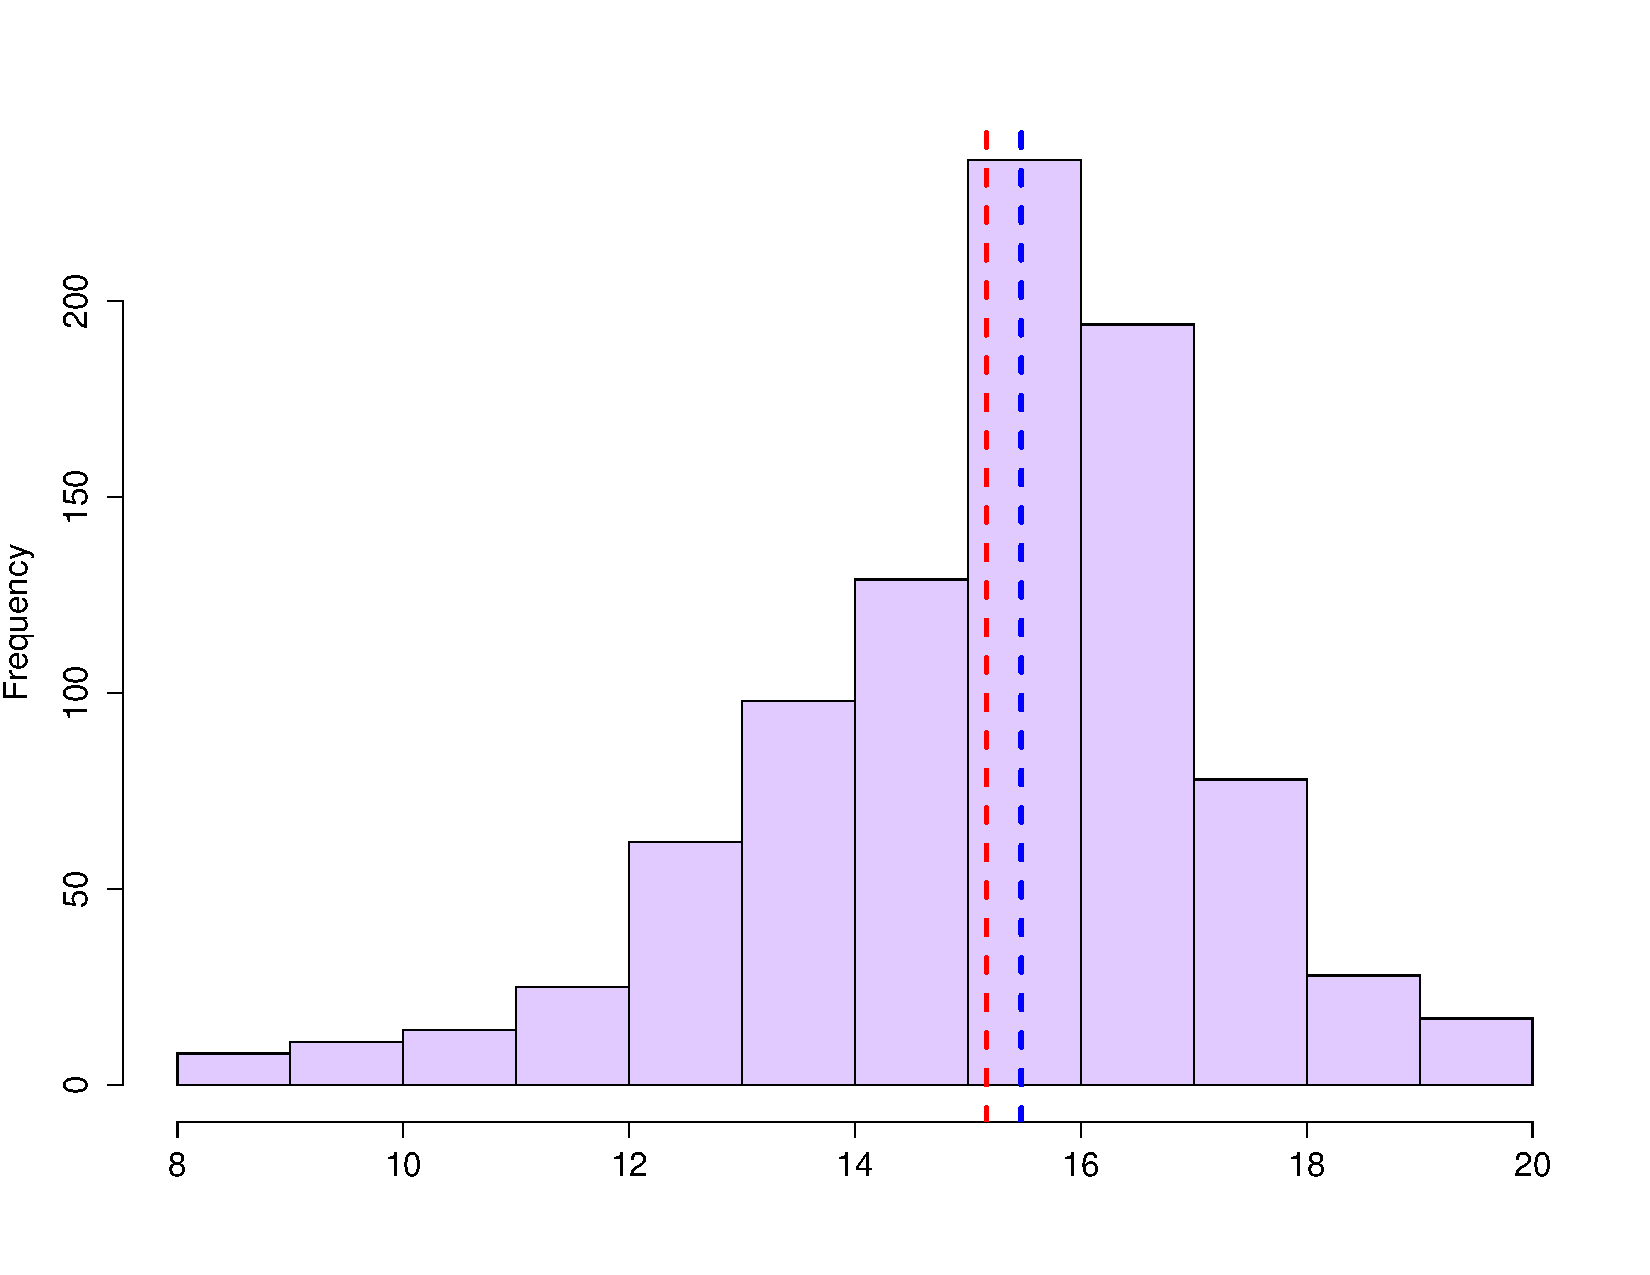
\includegraphics[scale=0.325]{skew_left.pdf} } 
\put(225,150){\hbox{mean	\quad\quad	median}}
\end{picture}

\end{frame}



%\subsection*{Skewness}

\begin{frame}
\frametitle{Skewness Ctd...}

%\vspace{-0.10cm}
\underline{None of the above}
(i.e. can not determine skewness visually)

\begin{picture}(200,200)
\put(0,0){ 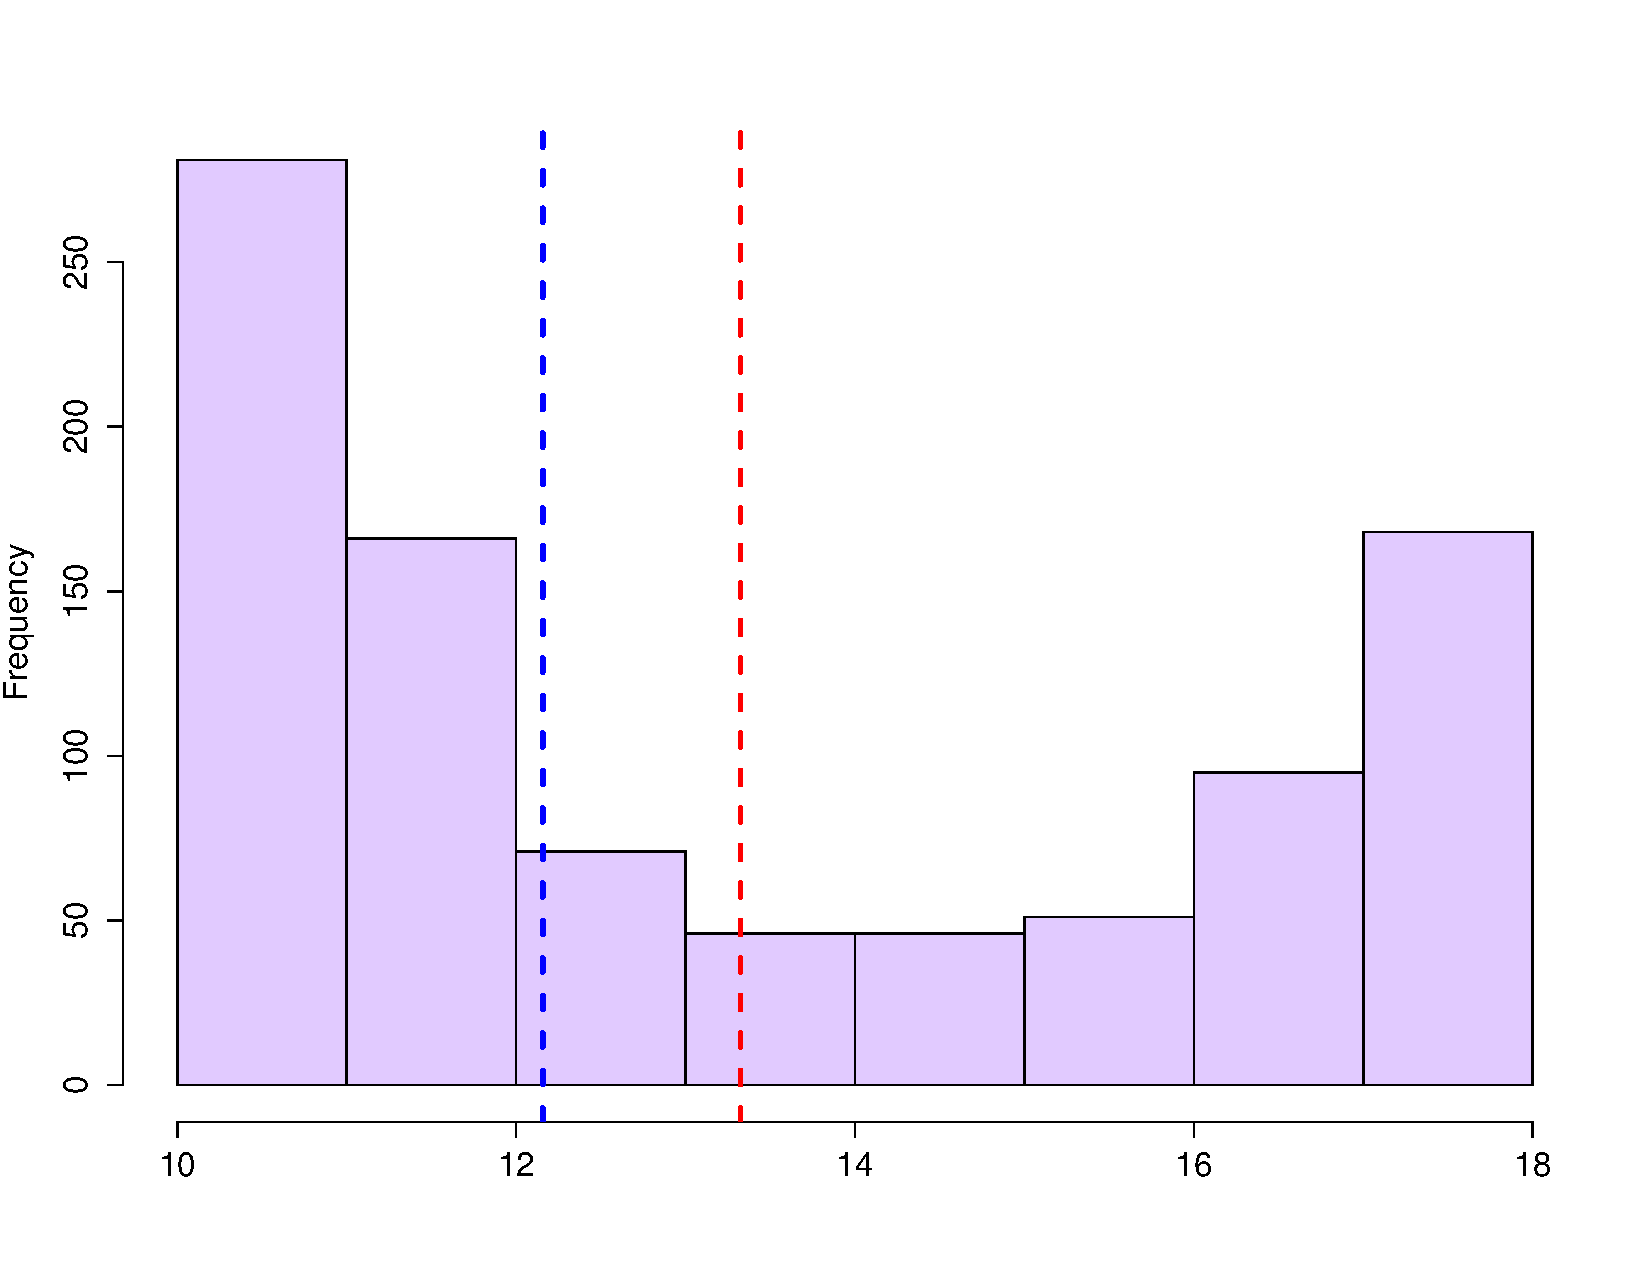
\includegraphics[scale=0.325]{neither.pdf} } 
% \put(225,150){\hbox{mean	\quad\quad	median}}
\end{picture}

\end{frame}



%\subsection*{Percentiles}

\begin{frame}
\frametitle{Percentiles}

\begin{definition}[Percentile]
\justifying
For ordered data the $p^{th}$ percentile is a value such that p\% of observer data fall below it.
\end{definition}

\begin{itemize}
\item	We are particularly interested in:
	\begin{itemize}
	\item	The 25$^{\text{th}}$ percentile
	\item	The 50$^{\text{th}}$ percentile (median)
	\item	The 75$^{\text{th}}$ percentile
	\end{itemize}
\hfill\\
\vspace{0.25cm}
\item	We call these values \alert{quartiles}.
\end{itemize}

\end{frame}



%\subsection*{Quartiles}

\begin{frame}
\frametitle{Quartiles}

\vspace{0.5cm}

\hspace*{-22.5pt}
\begin{tabular}{L{2.55cm} C{0.12cm} l}
First Quartile	& : &		A value such that 25\% of observations lie below it.	\\
(Q$_{1}$)		&   &		\hspace{2.5cm} \scriptsize{(a quarter)}	\hspace{2cm}	\scriptsize{(25$^{\text{th}}$ percentile)} \\
\hfill\\
Second Quartile	& : &		A value such that 50\% of observations lie below it.	\\
(Q$_{2}$)			&   &		\hspace{2.5cm} \scriptsize{(two quarters)}		\hspace{1.55cm}	\scriptsize{(50$^{\text{th}}$ percentile)} \\
(median)			&   &		\\
\hfill\\
Third Quartile	& : &		A value such that 75\% of observations lie below it.	\\
(Q$_{3}$)		&   &		\hspace{2.5cm} \scriptsize{(three quarters)}	\hspace{1.3cm}	\scriptsize{(75$^{\text{th}}$ percentile)} \\
\end{tabular}
\hfill\\
\hfill\\
\hfill\\

The \alert{inter-quartile range (IQR)} is: \\

\begin{center}
IQR =  Q$_{3}$ --- Q$_{1}$
\end{center}

\end{frame}



%\subsection*{Quartiles}
\begin{frame}
\frametitle{Quartiles Ctd...}

\textbf{Note:}

\begin{itemize}
\item	The ``interquartile range'' should \underline{not} be confused with the ``\alert{range}''. \\
\hfill\\
\item	The \alert{range} is defined as\\
	\begin{center}
	Range = max --- min
	\end{center}
\end{itemize}

\end{frame}




%\subsection*{Example}

\begin{frame}[t]
\frametitle{Example}
Find the quartiles and interquartile range for the set of data below:

\begin{center}
109, ~112, ~114, ~120, ~126, ~132, ~141, ~142, ~147, ~150, ~152
\end{center}

\end{frame}



%\subsection*{Boxplots}

\begin{frame}
\frametitle{Boxplots}

\vspace{-1.0cm}

\begin{itemize}
\justifying
\item	Boxplots are another visual aid to present data.\\
\hfill\\
\item	We use the quartiles as well as:\\
\hfill\\
	\begin{tabular}{lcl}
	Lower Whisker	& : &		Q$_{1}$ --- 1.5(IQR)		\\
	\hfill\\
	Upper Whisker	& : &		Q$_{3}$ + 1.5(IQR)
	\end{tabular}
\hfill\\
\hfill\\
\vspace{0.25cm}
\item	Boxplots are useful in helping us identify \alert{outliers}.\\
\hfill\\
\item An \alert{outlier} is an unusual data point that appears to be far away from the rest of the data.
	(i.e. it appears outside the range that we would expect to see ``typical'' values of the data we are studying. 
\end{itemize}

\end{frame}



%\subsection*{Boxplots}

\begin{frame}
\frametitle{Boxplots Ctd...}

%How to interpret a Boxplot
%
\vspace{-0.60cm}

\hspace*{12pt}
\begin{picture}(175,230)
\put(0,0){ 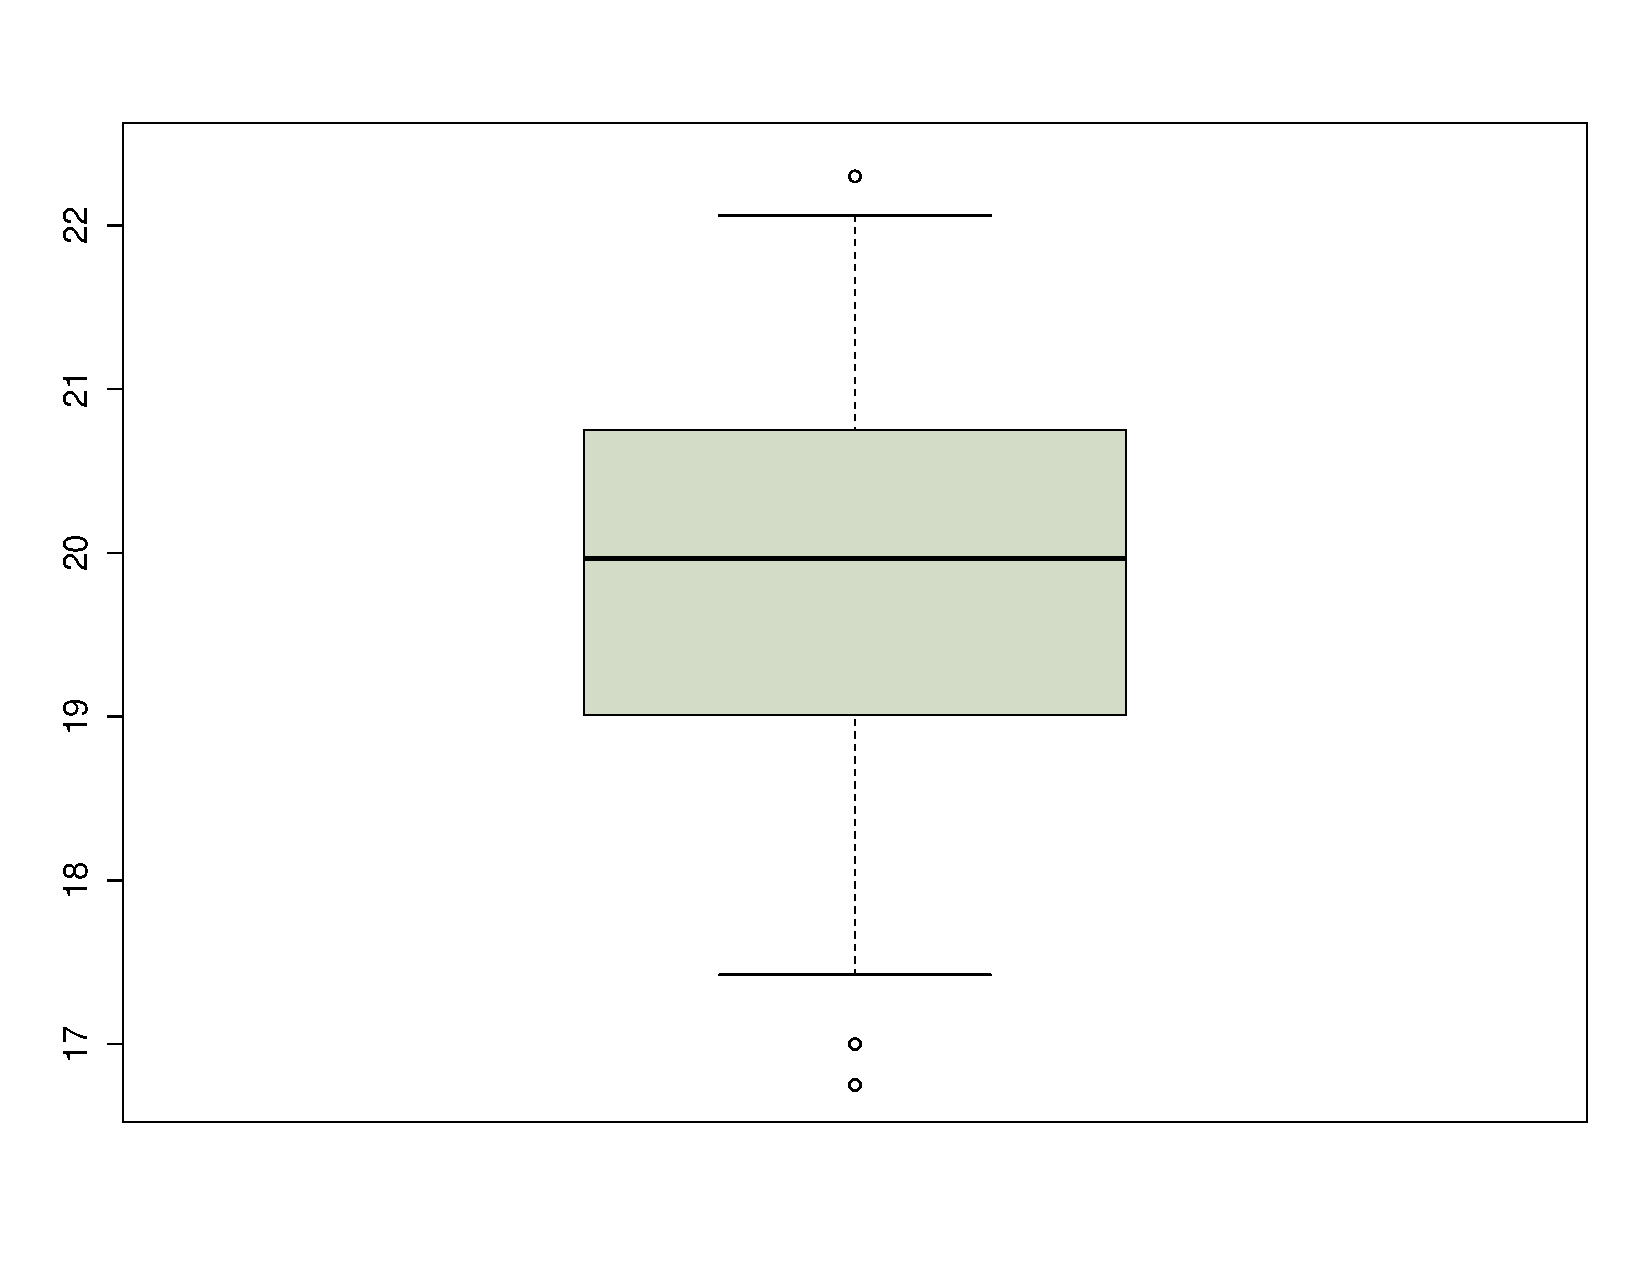
\includegraphics[scale=0.350]{boxplot.pdf} } 

\put(-25,140){\hbox{ \scriptsize{Q$_{3}$} } }
\put(-25,118){\hbox{ \scriptsize{Q$_{2}$} } }
\put(-25,93){\hbox{ \scriptsize{Q$_{1}$} } }

\put(176,48){\hbox{ \scriptsize{Q$_{1} $} --- 1.5(IQR) } }
\put(176,178){\hbox{ \scriptsize{Q$_{3} $} + 1.5(IQR) } }

\put(150, 32.5){ $\}$ }
\put(155.0,33.0){ \hbox{ \scriptsize{outliers} } }

\put(135.5,183.0){ $\{$ }
\put(104,184){ \hbox{ \scriptsize{outliers} } }


\put(-10, 215.0){ \hbox{How to interpret a boxplot } }

%\put(225,150){\hbox{mean	\quad\quad	median}}
\end{picture}

\begin{tikzpicture}[overlay]
\draw [dashed] (0.25, 5.42) -- (5, 5.42);
\draw [dashed] (0.25, 4.66) -- (5, 4.66);
\draw [dashed] (0.25, 3.74) -- (5, 3.74);
\end{tikzpicture}

\end{frame}



%\subsection*{Boxplots}
\begin{frame}[t]
\frametitle{Boxplots Ctd...}

\small

\vspace{-0.25cm}
\begin{itemize}
\justifying
\item	We can sometimes the get information about skewness of data from a boxplot.\\
%\hfill\\
%\vspace{-0.1cm}
\item	Consider the following 3 boxplots.
\end{itemize}
\vspace{-0.45cm}
\begin{center}
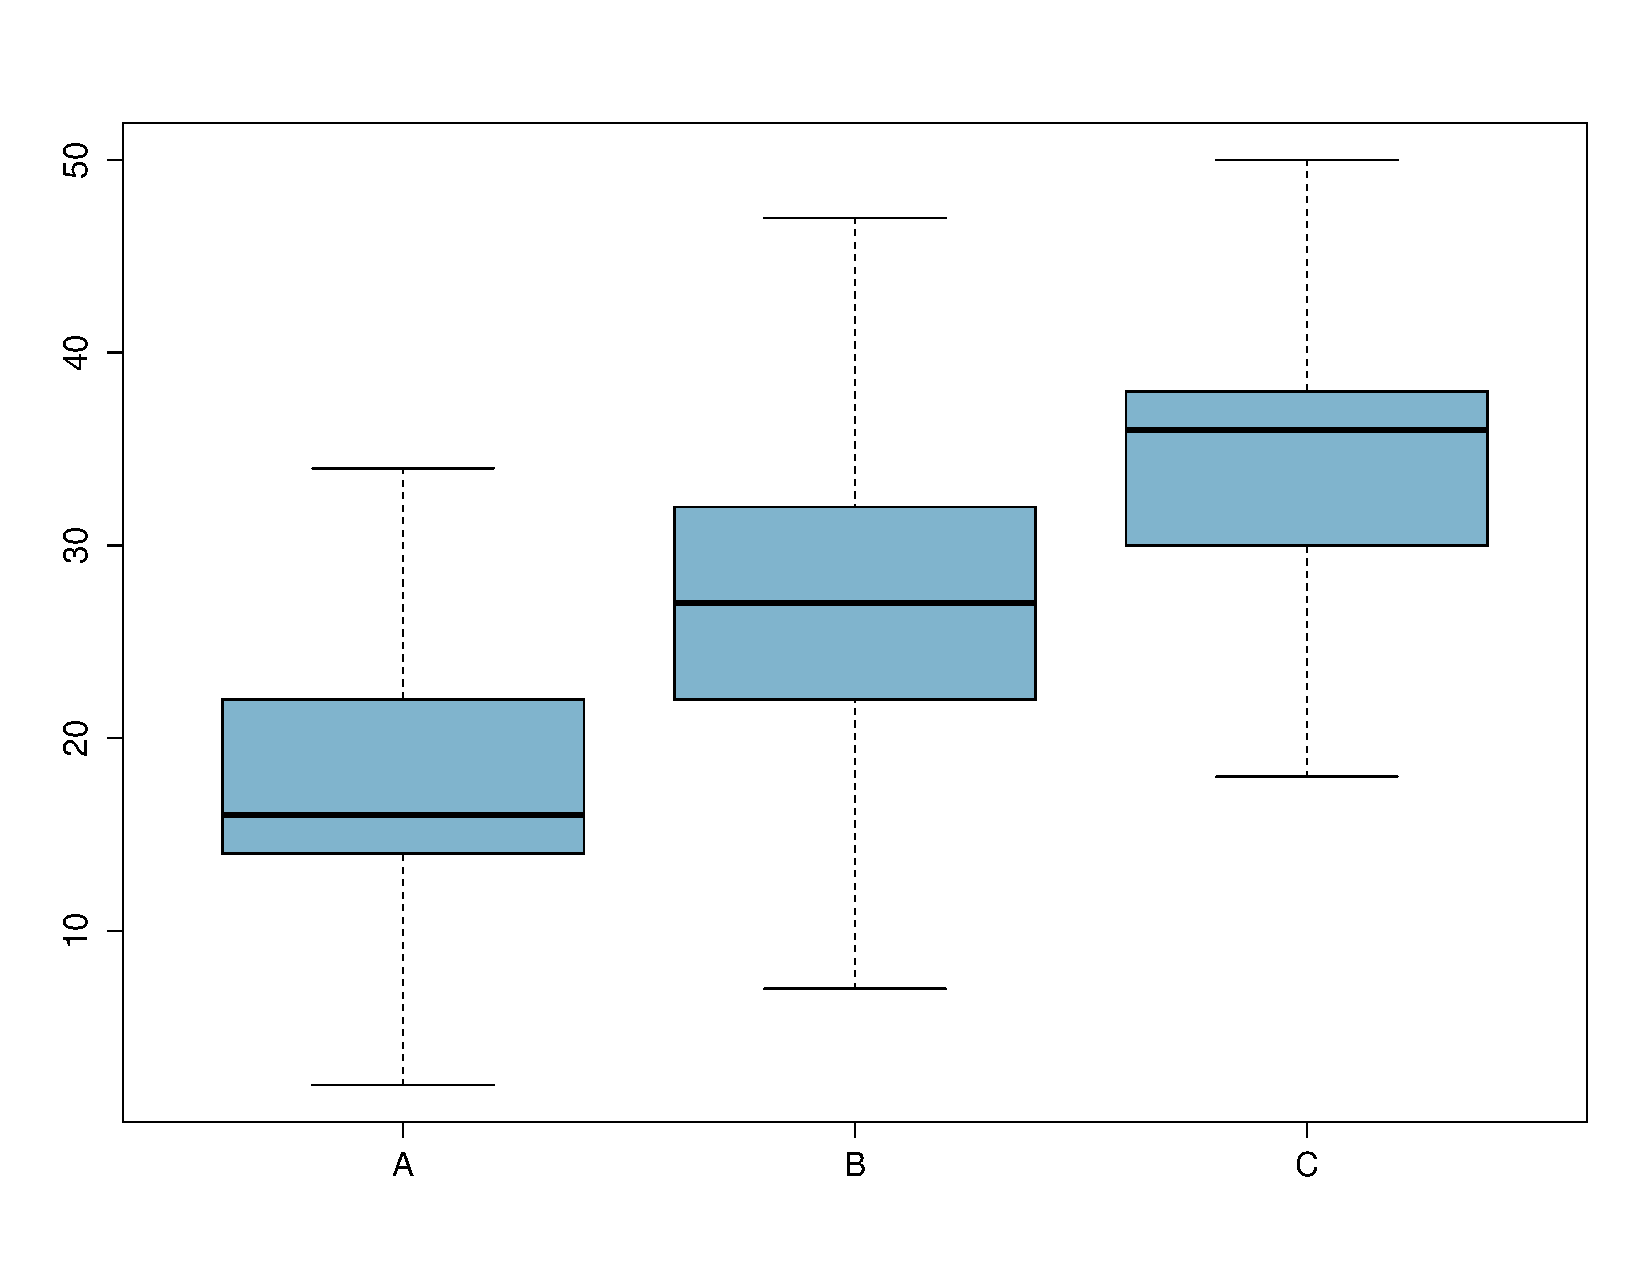
\includegraphics[scale=0.265]{boxplot_abc.pdf}
\end{center}

\end{frame}



%\subsection*{Boxplots}
\begin{frame}[t]
\frametitle{Boxplots Ctd...}

\vspace{-0.80cm}

\hspace*{-10pt}

\hspace*{-25pt}
\begin{tikzpicture}%[overlay]
	\node at (2.5, -2) { 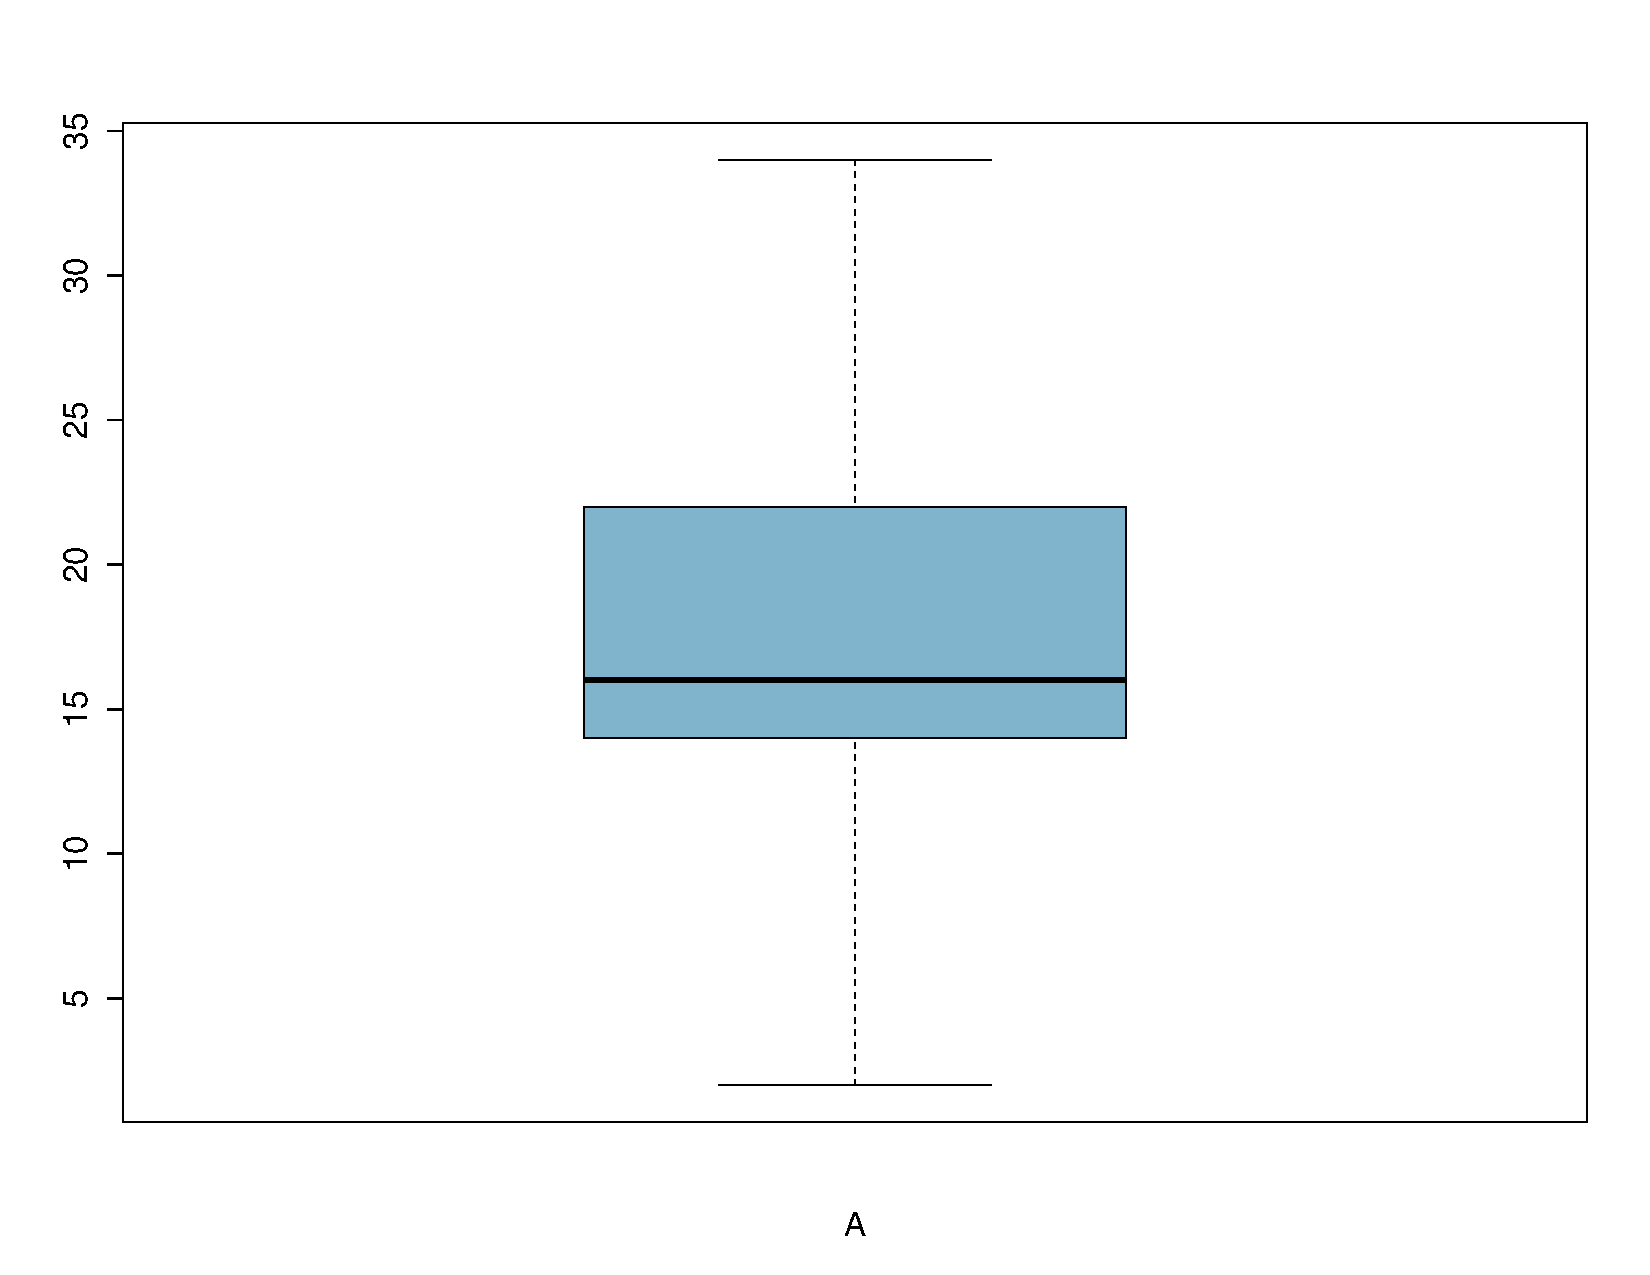
\includegraphics[scale=0.23]{boxplot_A.pdf} };
	\node at (8.65,  -5.1) { 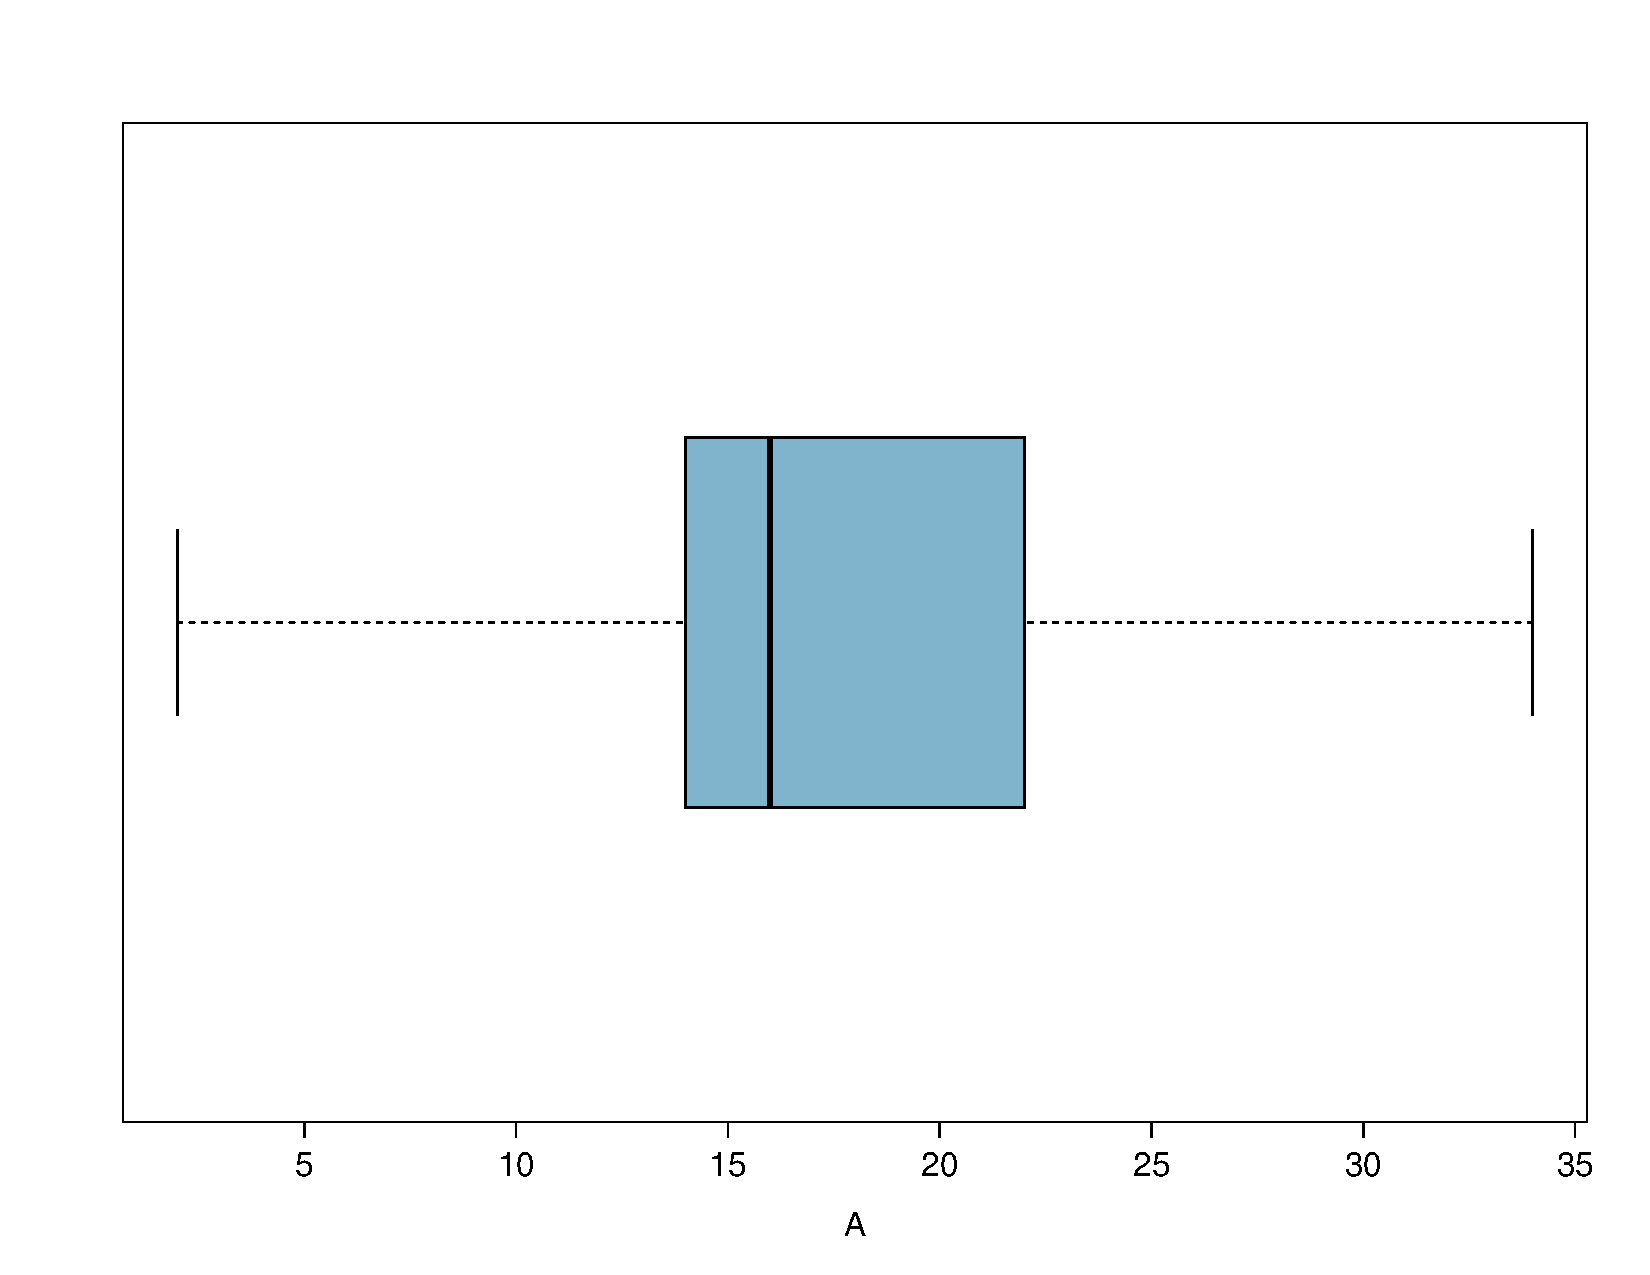
\includegraphics[width=6.20cm,height=2.5cm]{boxplot_A_horiz.pdf} };
	\draw[draw=black,color=black] (6,-3.90) rectangle (11.5,0.00);
\end{tikzpicture}

\begin{picture}(200,200)
\put(-15, 392){\hbox{ \underline{Boxplot} }}
\put(168, 392){\hbox{ \underline{Distribution} }}
\end{picture}

\end{frame}




%\subsection*{Boxplots}
\begin{frame}[t]
\frametitle{Boxplots Ctd...}

\vspace{-0.80cm}

\hspace*{-10pt}

\hspace*{-25pt}
\begin{tikzpicture}%[overlay]
	\node at (2.5, -2) { 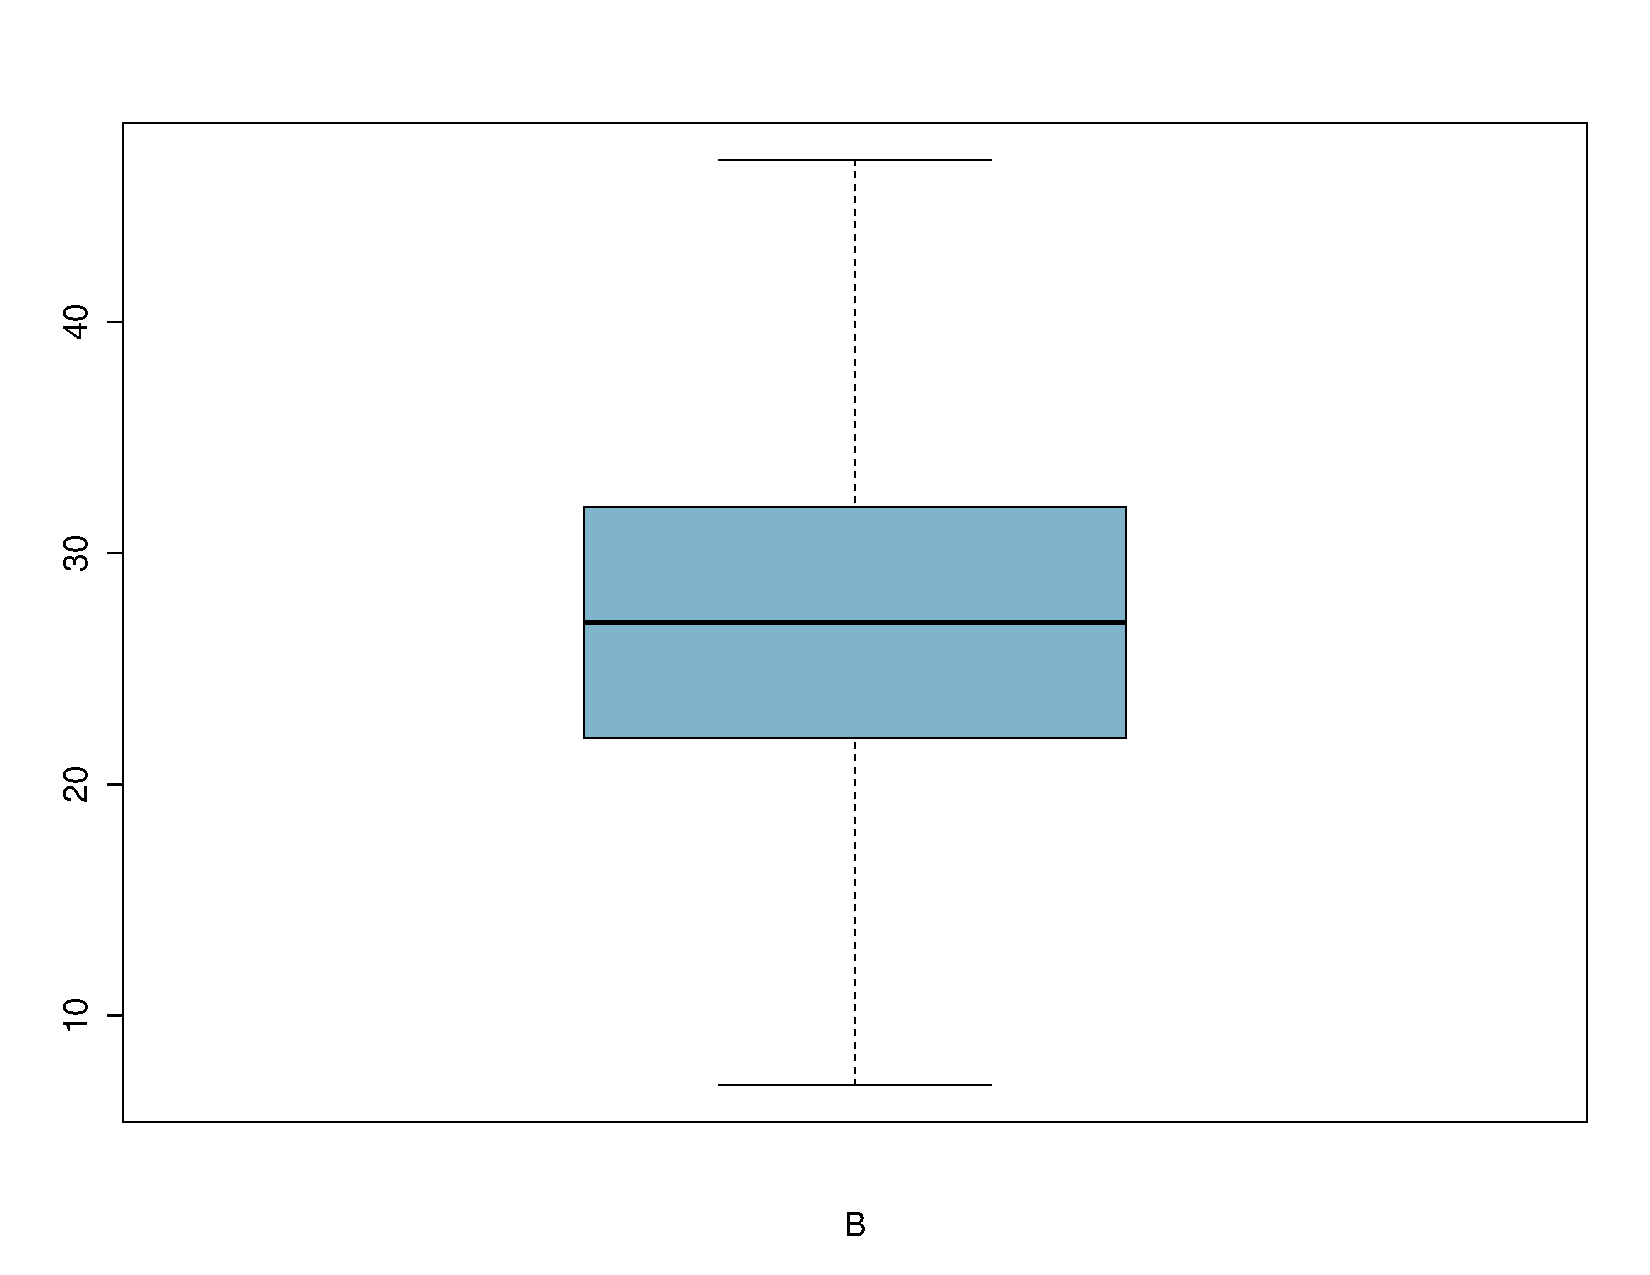
\includegraphics[scale=0.23]{boxplot_B.pdf} };
	\node at (8.65,  -5.1) { 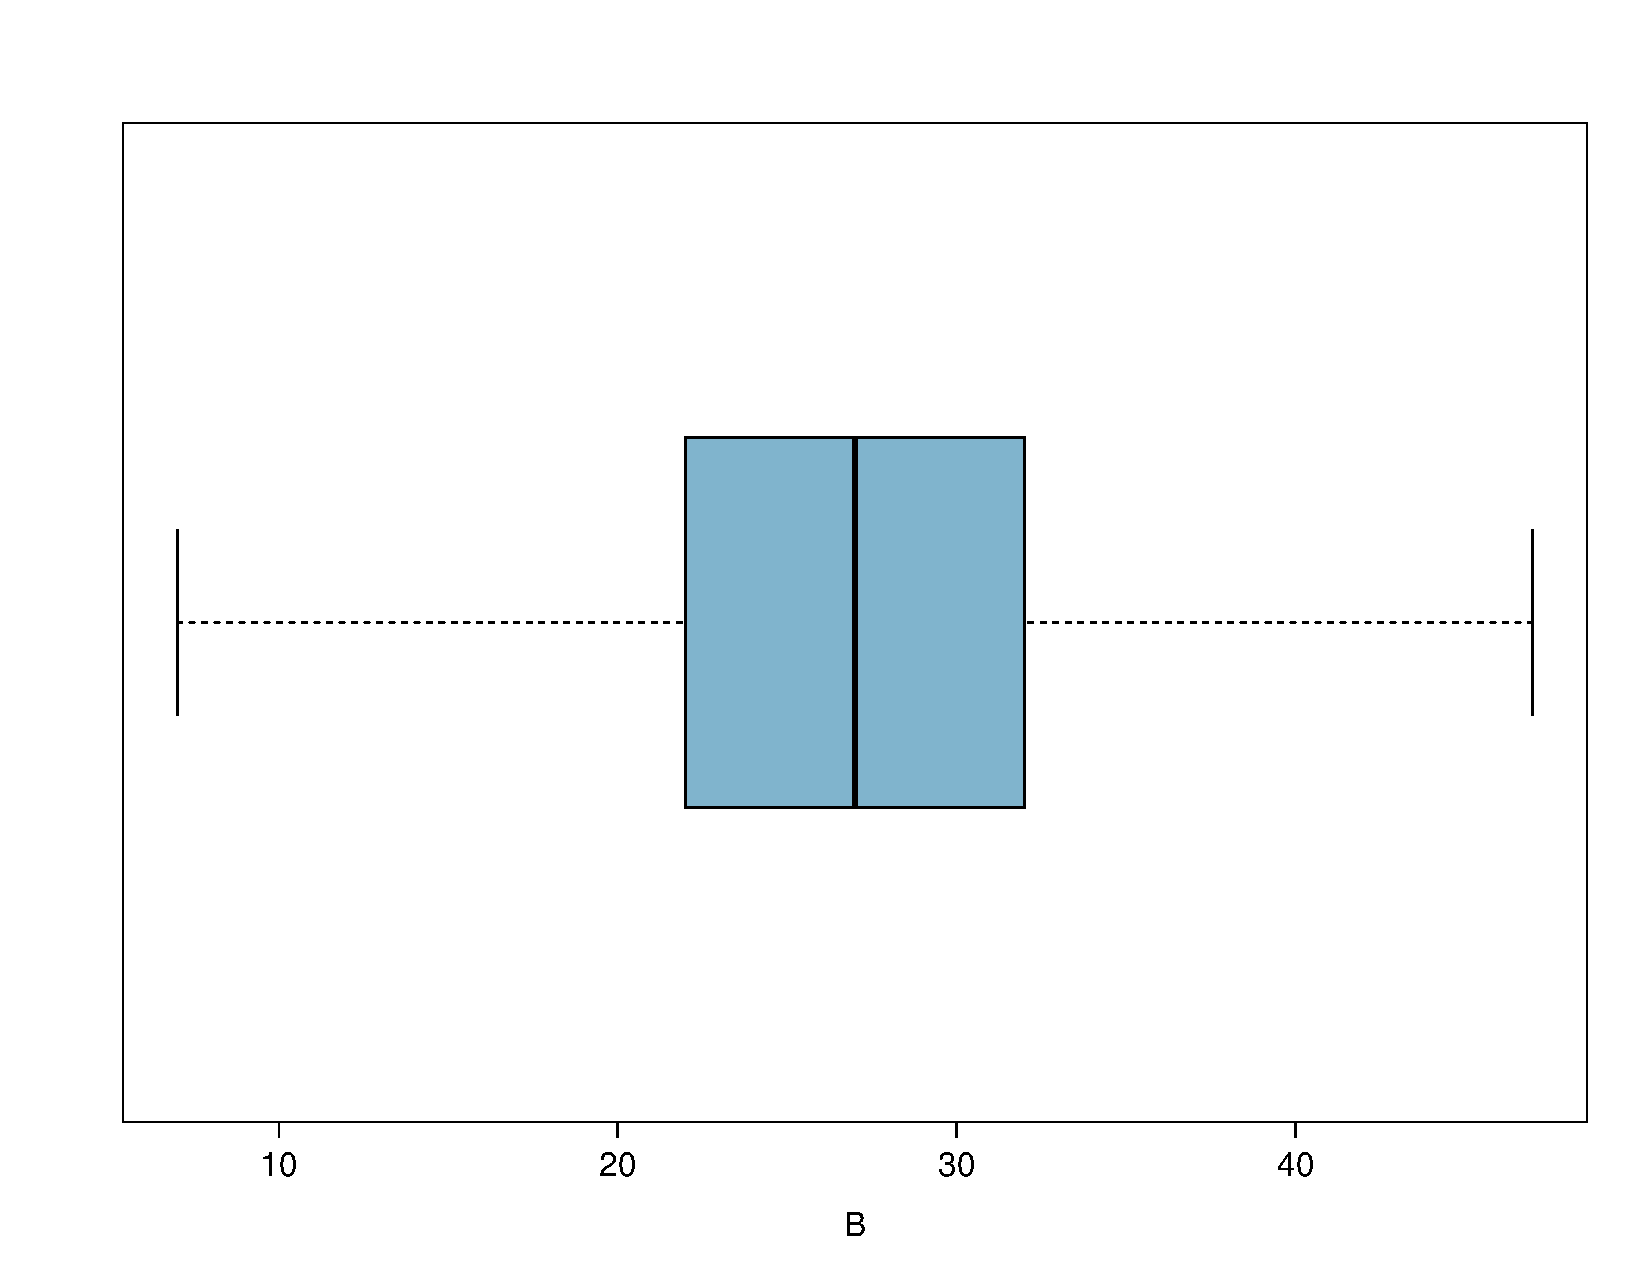
\includegraphics[width=6.20cm,height=2.5cm]{boxplot_B_horiz.pdf} };
	\draw[draw=black,color=black] (6,-3.90) rectangle (11.5,0.00);
\end{tikzpicture}

\begin{picture}(200,200)
\put(-15, 392){\hbox{ \underline{Boxplot} }}
\put(168, 392){\hbox{ \underline{Distribution} }}
\end{picture}

\end{frame}




%\subsection*{Boxplots}
\begin{frame}[t]
\frametitle{Boxplots Ctd...}

\vspace{-0.80cm}

\hspace*{-10pt}

\hspace*{-25pt}
\begin{tikzpicture}%[overlay]
	\node at (2.5, -2) { 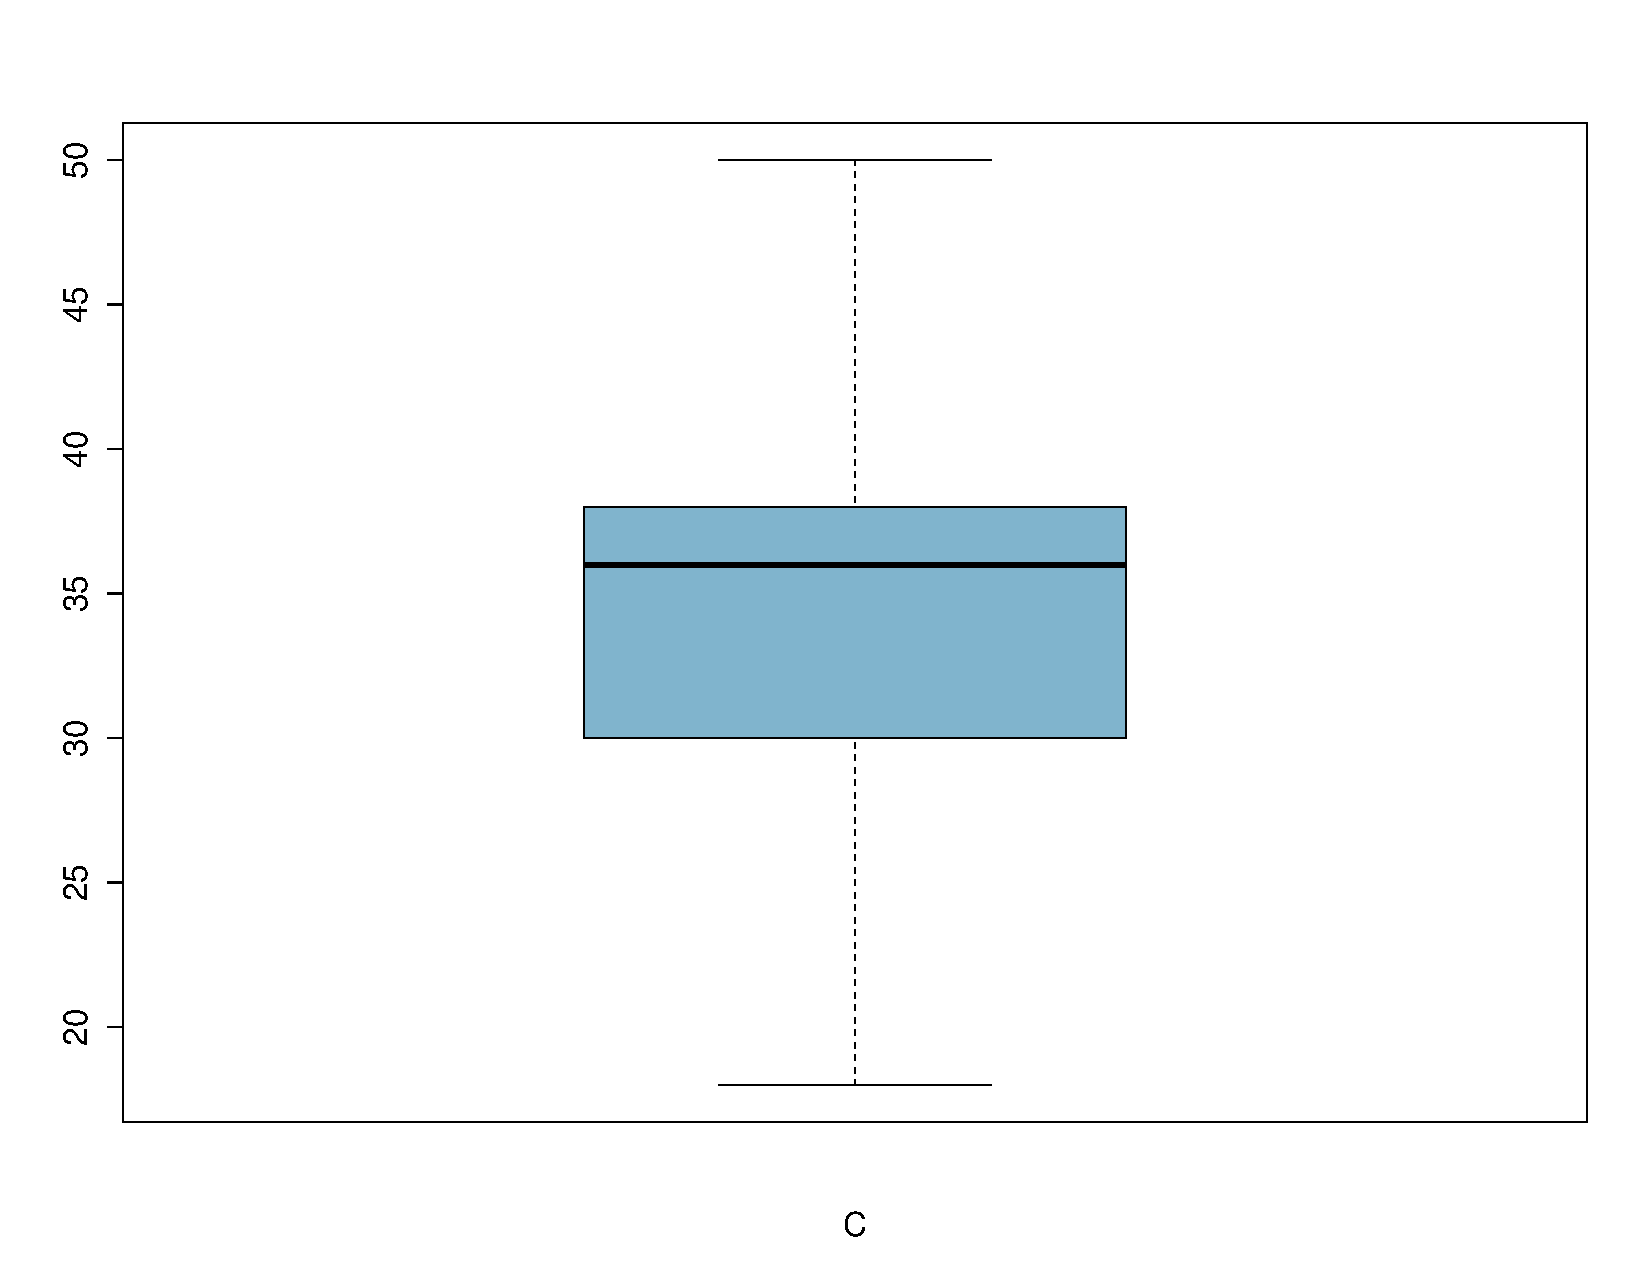
\includegraphics[scale=0.23]{boxplot_C.pdf} };
	\node at (8.65,  -5.1) { 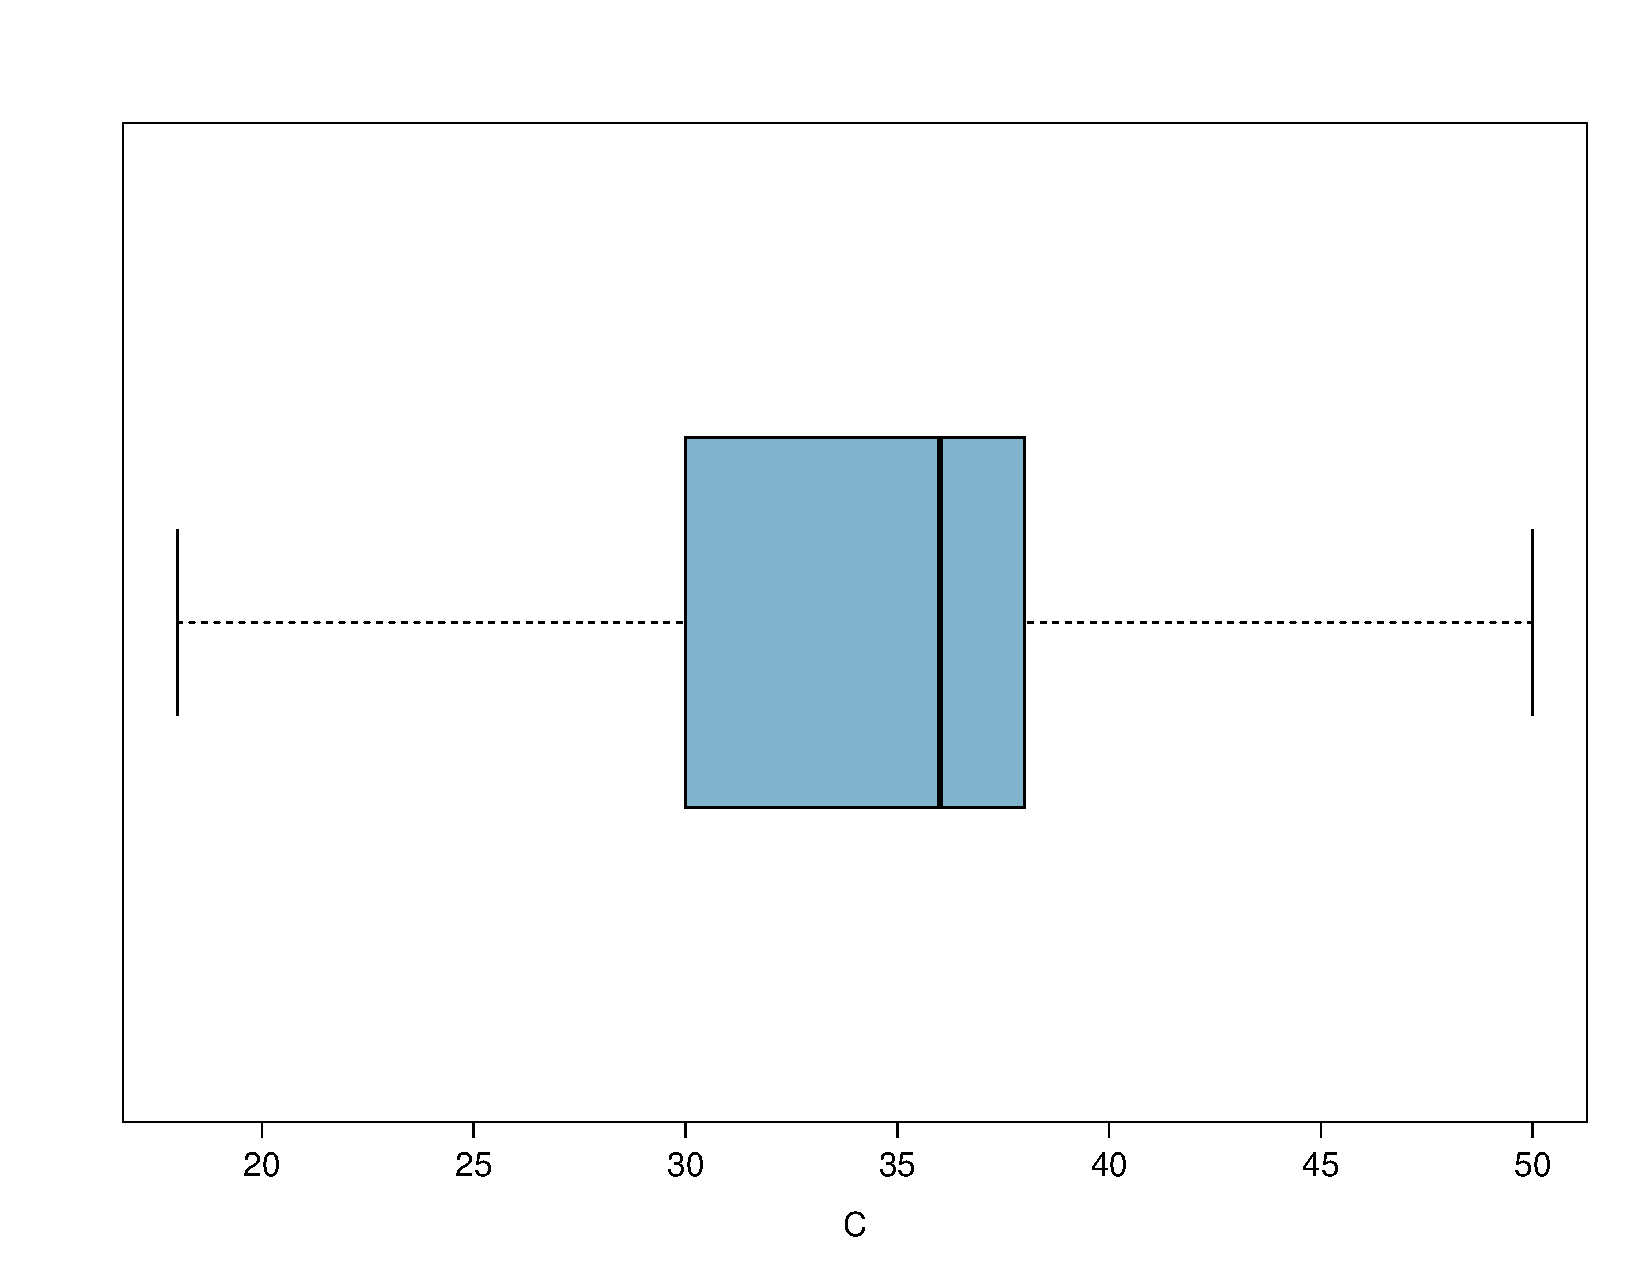
\includegraphics[width=6.20cm,height=2.5cm]{boxplot_C_horiz.pdf} };
	\draw[draw=black,color=black] (6,-3.90) rectangle (11.5,0.00);
\end{tikzpicture}

\begin{picture}(200,200)
\put(-15, 392){\hbox{ \underline{Boxplot} }}
\put(168, 392){\hbox{ \underline{Distribution} }}
\end{picture}

\end{frame}


%\subsection*{Stem and Leaf Plots}

\begin{frame}
\frametitle{Stem and Leaf Plots}

\begin{itemize}
\justifying
\item	A \alert{Stem and leaf} plot (also known as a \alert{stem plot}), is a tabular method to display data.\\
\hfill\\
\item	Each observation is split into a stem (the ``larger'' part of an observation) and a ``leaf'' (the smaller part of an observation).\\
\hfill\\
\item	One common partition is to use the stem as a whole number and the leaves as the decimal part of the number.
	Another common partition is to consider the stem to be the integer part of some power of 10 (ex. 10, 100, 1000 etc.).\\
\hfill\\
\item	Stem and leaf plots are easier to understand with the aid of an example.
\end{itemize}

\end{frame}




%\subsection*{Stem and Leaf Plots}

\begin{frame}
\frametitle{Stem and Leaf Plots ctd.}

\footnotesize

\vspace{-0.250cm}

\begin{itemize}
\item	For example consider the following set of (sorted) data points:\\
	\hfill\\
	\hspace*{-20pt}
	\begin{tabular}{c c c c c c c c c c}
	10.1	&	10.1	&	10.2	&	10.3	&	11.1	&	11.2	&	11.2	&	11.2	&	11.3	&	12.0	\\ 
	12.0	&	12.3	&	12.4	&	12.5	&	12.5	&	12.6	&	14.2	&	14.2	&	14.3	&	14.3	\\
	14.4	&	15.1	&	15.2	&	15.3	&	15.3	&	16.0	&	16.1	&	16.2	&	 18.0	&	18.1
	\end{tabular}
\hfill\\
\vspace{0.25cm}
\item	Let's group terms and rewrite our data as follows:\\
\hfill\\
\begin{center}
\begin{tabular}{c c c c c c c c c c}
10.1	&	10.1	&	10.2	&	10.3	\\ 
11.1	&	11.2	&	11.2	&	11.2	&	11.3	\\
12.0	&	12.0	&	12.3	&	12.4	&	12.5	&	12.5	&	12.6	\\
14.2	&	14.2	&	14.3	&	14.3	&	14.4	\\	
15.1	&	15.2	&	15.3	&	15.3	\\
16.0	&	16.1	&	16.2	\\
18.0	&	18.1	\\
\end{tabular}
\end{center}
\hfill\\
\item	We can now construct out stem and leaf plot. 
\end{itemize}

\end{frame}






%\subsection*{Stem and Leaf Plots}

\begin{frame}
\frametitle{Stem and Leaf Plots ctd.}

%\vspace{-0.200cm}

\footnotesize

\begin{center}
\begin{tabular}{c c c c c c c c c c}
10.1	&	10.1	&	10.2	&	10.3	\\ 
11.1	&	11.2	&	11.2	&	11.2	&	11.3	\\
12.0	&	12.0	&	12.3	&	12.4	&	12.5	&	12.5	&	12.6	\\
14.2	&	14.2	&	14.3	&	14.3	&	14.4	\\	
15.1	&	15.2	&	15.3	&	15.3	\\
16.0	&	16.1	&	16.2	\\
18.0	&	18.1	\\
\end{tabular}
\end{center}
\vspace{-0.250cm}
\begin{itemize}
\item	Let's choose our partition ($|$) to be at the decimal point:
\end{itemize}
\hspace{0.75cm} Stem and Leaf Plot:
\vspace{-0.30cm}
\begin{center}
\begin{tabular}{r c l}
%\hfill\\
10	&	$|$	&	1123		\\
11	&	$|$	&	12223	\\
12	&	$|$	&	0034556	\\
13	&	$|$	&			\\
14	&	$|$	&	22334	\\
15	&	$|$	&	1233		\\
16	&	$|$	&	012		\\
17	&	$|$	&			\\
18	&	$|$	&	01		\\
\end{tabular}
\end{center}

\end{frame}






\section{Homework}

\subsection*{Homework}

\begin{frame}
\frametitle{Homework}

\vspace{-0.5cm}

\textbf{Readings}

\begin{itemize}\justifying
\item	Introduction to Probability and Statistics:\\
	\quad Read 2.1.1 --- 2.2.2 ~(Pages 23 --- 34)
\end{itemize}

\hfill\\

\textbf{Exercises}

\begin{itemize}\justifying
\item	Custom Edition of Statistics for Business and Economics (McClave, Benson, Sincich):\\
	\quad Exercises 2.35 --- 2.41 \\
\hfill\\
\item	11$^{\text{th}}$ Edition of Statistics for Business and Economics (McClave, Benson, Sincich):\\
	\quad Exercises 2.33 --- 2.36	\\
\end{itemize}




\end{frame}





\end{document}

